%%%%%%%%%%%%%%%%%%%%%%%%%%%%%%%%%%%%%%%%%%%%%%%%%%%%%%%%%%%%%%%%%%%%%%%%%%%%
%% Author template for Marketing Science (mksc)
%% Mirko Janc, Ph.D., INFORMS, mirko.janc@informs.org
%% ver. 0.95, December 2010
%%%%%%%%%%%%%%%%%%%%%%%%%%%%%%%%%%%%%%%%%%%%%%%%%%%%%%%%%%%%%%%%%%%%%%%%%%%%
\documentclass[mksc,blindrev]{informs3} % current default for manuscript submission
%\documentclass[mksc,nonblindrev]{informs3}

%%\OneAndAHalfSpacedXI % current default line spacing
\OneAndAHalfSpacedXII
%%\DoubleSpacedXII
%%\DoubleSpacedXI

% If hyperref is used, dvi-to-ps driver of choice must be declared as
%   an additional option to the \documentclass. For example
%\documentclass[dvips,mksc]{informs3}      % if dvips is used
%\documentclass[dvipsone,mksc]{informs3}   % if dvipsone is used, etc.

% Private macros here (check that there is no clash with the style)
\usepackage{subcaption}
% Natbib setup for author-year style
\usepackage{natbib}
 \bibpunct[, ]{(}{)}{,}{a}{}{,}%
 \def\bibfont{\small}%
 \def\bibsep{\smallskipamount}%
 \def\bibhang{24pt}%
 \def\newblock{\ }%
 \def\BIBand{and}%


%% Setup of theorem styles. Outcomment only one. 
%% Preferred default is the first option.
\TheoremsNumberedThrough     % Preferred (Theorem 1, Lemma 1, Theorem 2)
%\TheoremsNumberedByChapter  % (Theorem 1.1, Lema 1.1, Theorem 1.2)

%% Setup of the equation numbering system. Outcomment only one.
%% Preferred default is the first option.
\EquationsNumberedThrough    % Default: (1), (2), ...
%\EquationsNumberedBySection % (1.1), (1.2), ...
\DeclareMathOperator{\logit}{logit}
% In the reviewing and copyediting stage enter the manuscript number.
%\MANUSCRIPTNO{} % When the article is logged in and DOI assigned to it,
                 %   this manuscript number is no longer necessary

%%%%%%%%%%%%%%%%
\begin{document}
%%%%%%%%%%%%%%%%

% Outcomment only when entries are known. Otherwise leave as is and 
%   default values will be used.
%\setcounter{page}{1}
%\VOLUME{00}%
%\NO{0}%
%\MONTH{Xxxxx}% (month or a similar seasonal id)
%\YEAR{0000}% e.g., 2005
%\FIRSTPAGE{000}%
%\LASTPAGE{000}%
%\SHORTYEAR{00}% shortened year (two-digit)
%\ISSUE{0000} %
%\LONGFIRSTPAGE{0001} %
%\DOI{10.1287/xxxx.0000.0000}%

% Author's names for the running heads
% Sample depending on the number of authors;
% \RUNAUTHOR{Jones}
% \RUNAUTHOR{Jones and Wilson}
% \RUNAUTHOR{Jones, Miller, and Wilson}
% \RUNAUTHOR{Jones et al.} % for four or more authors
% Enter authors following the given pattern:
%\RUNAUTHOR{}

% Title or shortened title suitable for running heads. Sample:
% \RUNTITLE{Bundling Information Goods of Decreasing Value}
% Enter the (shortened) title:
%\RUNTITLE{}

% Full title. Sample:
% \TITLE{Bundling Information Goods of Decreasing Value}
% Enter the full title:
%\TITLE{}

% Block of authors and their affiliations starts here:
% NOTE: Authors with same affiliation, if the order of authors allows, 
%   should be entered in ONE field, separated by a comma. 
%   \EMAIL field can be repeated if more than one author
\ARTICLEAUTHORS{%
\AUTHOR{Eric Schwartz}
\AFF{University of Michigan, \EMAIL{}, \URL{}}
\AUTHOR{Kenneth Fairchild}
\AFF{Sawtooth Software, \EMAIL{}, \URL{}}
\AUTHOR{Bryan Orme}
\AFF{Sawtooth Software, \EMAIL{}, \URL{}}
\AUTHOR{Alexander Zaitzeff}
\AFF{University of Michigan, \EMAIL{}, \URL{}}
% Enter all authors
} % end of the block

\ABSTRACT{%
For large MaxDiff studies whose main purpose is identifying the top few items for the sample, a new adaptive approach called Bandit MaxDiff may increase efficiency fourfold over standard non-adaptive MaxDiff.  Bandit MaxDiff leverages information from previous respondents via aggregate logit and Thompson Sampling so later respondents receive designs that oversample the topmost items that are most likely to turn out to be the overall winners. 
Keywords: Active learning, adaptive conjoint, multi-armed bandit, best-worst scaling, MaxDiff, Thompson Sampling % Enter your abstract
}%

% Sample
%\KEYWORDS{deterministic inventory theory; infinite linear programming duality; 
%  existence of optimal policies; semi-Markov decision process; cyclic schedule}

% Fill in data.
\KEYWORDS{}

\maketitle
%%%%%%%%%%%%%%%%%%%%%%%%%%%%%%%%%%%%%%%%%%%%%%%%%%%%%%%%%%%%%%%%%%%%%%

% Samples of sectioning (and labeling) in MKSC
% NOTE: (1) \section and \subsection do NOT end with a period
%       (2) \subsubsection and lower need end punctuation
%       (3) capitalization is as shown (title style).
%
%\section{Introduction.}\label{intro} %%1.
%\subsection{Duality and the Classical EOQ Problem.}\label{class-EOQ} %% 1.1.
%\subsection{Outline.}\label{outline1} %% 1.2.
%\subsubsection{Cyclic Schedules for the General Deterministic SMDP.}
%  \label{cyclic-schedules} %% 1.2.1
%\section{Problem Description.}\label{problemdescription} %% 2.

% Text of your paper here
\section{Introduction}

Firms collect more customer data than ever. While much of that is behavioral data (e.g., purchases, clicks, visits, etc.), the online market research relies on surveys (e.g., preference measurement) at an increasingly large scale. And as firms push preference measurement methods into a larger scale, market researchers seek to collect data as efficiently. \\
One common managerial decision driving such data collection is to select which are most preferred among a large set of hundreds of possible items. For instance, consider these illustrative managerial decisions: select which features should we offer in a new product; select the most preferred levels of a product attribute; and select the consumer benefits we should emphasize in marketing communications.  For each problem, a market researcher may have to screen out hundreds of ``items'' (e.g., features, benefits, messages).\\
But typical choice experiment methods, such as conjoint, are infeasible for cost or simply inefficient at this scale. Instead, researchers often use pretest or screening phases to select a smaller set, and use that for the main analysis. Yet there is no systematic method to smoothly transition out of that screening phase, even when the ultimate objective is learning precisely the set of most preferred items. \\
Choice experiment methods for preference measurement continue to be among the most widely adopted market research methods. Choice-based conjoint (CBC) analysis and maximum difference (MaxDiff), for instance, are common choice tasks that continue to be used in both academic and industry settings.\\
Methodological advances, such as adaptive conjoint, have long sought to improve efficiency, obtaining more information from fewer respondents. Those methods will use past responses to select the next question to improve precision of all parameters. For instance, adaptive choice-based conjoint (ACBC) methods present respondents with questions to reduce the uncertainty where it is greatest. It chooses the next question to best reduce overall uncertainty.\\
But the market researcher's goal is typically not to obtain precise estimates of utility of every single alternative or attribute level. If their goal is to identify the most preferred items, why do they need to spend resources (questions, respondents, time) to learn how precisely poor the least-preferred item is compared to the second-least preferred item? \\
With that objective in mind, we propose a new adaptive choice experiment method. 
Our approach departs from traditional adaptive survey methods like adaptive conjoint analysis (ACA). They aim to improve the precision of each of the parameters; we estimate the best items more precisely. \\
We propose a new adaptive method, combining MaxDiff and multi-armed bandit methods, as an example of an even broader framework for stated choice data collection. The focus of our research is a broader framework to align the data collection process with such managerial objectives. By aligning the two, we aim to improve efficiency and scalability for big data collection via choice experiments. We find we can ``get more for less,'' by improving precision using a smaller sample size compared to existing methods.\\
We propose this framework more broadly but will demonstrate it with MaxDiff, as it is an increasingly popular and important choice experiment method. But we will consider the general choice-based conjoint case in our discussion section. \\
UNDERLINED Our approach draws on state-of-the-art MAB algorithms in statistical machine learning called Follow The Perturbed Leader (FTPL) TO DO (Kalai and Vempala 2015). Recent theoretical advances prove that adding perturbations of Gumbel distributed noise leads to an optimal MAB strategy (Abernethy ,Lee, Tewari 2015; Kujala and Elomaa 2015). The perturbation methods provide an intuitive randomization decision strategy, which is appropriate for our application, yet their connection to other approaches and application have are limited. Perturbation not only resolves the explore-exploit (learn-earn) tradeoff for the stochastic (iid) bandit setting, but it also does so in the adversarial setting, suggesting it an MAB strategy more robust to changes in the non-random changes in the environment. We shed light on this methodological link as it has consequences beyond our method.\\
We contribute three ideas to the literature and practice. First, we frame choice task data collection as an earning-and-learning problem. During the process of data collection, we simultaneously balance the desire to learn preferences of all items and earn a reward towards achieving objective, by only serving questions the truly best subset of items. In this case, the objective is to identify the best set of items, for instance, the most desirable levels of attributes. The faster we identify the best items, the more we include them in questions, improving the precision of estimates. And if we need to reach a desired level of precision, we can do so faster, saving money in the form of number of respondents and time. 
Multi-armed bandit problems appear in marketing experiments for online advertising (Schwartz et al.; Urban et al.; Liberali et al.) and website design (Hauser et al.). One particular MAB method amenable to multi-variable parametric models is Thompson Sampling.\\
While we use bandit algorithms, our approach differs from extant bandit applications in a number of ways. For a bandit problem the reward is observed immediately (click, acquisition, purchase). While we have immediate observations (choice), that is not our reward. Instead, our goal is to correctly identify the truly best items as precisely as possible. These are not evaluable in real-time. \\
While our problem is not a bandit problem exactly, it is a bandit-inspired problem. However we find bandit algorithms form a heuristic to achieve our objective better than existing MaxDiff and conjoint methods. \\
Consider what would occur if the reward was whether an item is selected as best alternative, the arm's reward would be completely dependent on all of the other items presented in the set (e.g., was it presented alongside poor items). 
Second, the need to optimize this process is greater for large-scale problems with extremely large number of possible attribute levels or items.  In settings with hundreds of items, there is greater opportunity cost of focusing on items that are not important, calling for a need to improve efficiency.\\
Third, we propose an adaptive method for best-worst scaling. Existing adaptive methods have been largely limited to conjoint, adapting at both the aggregate level ~(Arora and Huber) and the individual level (Toubia et al). Yet best-worst methods, such as MaxDiff, have continued to emerge as important and commonly used in areas including marketing research and public health. We introduce a first step to make MaxDiff adaptive in a principled manner by using MAB methods. We accommodate an increasingly accepted method of solving multi-armed bandit problems, Thompson Sampling. We introduce two versions: MaxDiff - Thompson Sampling and its generalization MaxDiff $\epsilon$-diffuse Thompson Sampling.\\
The rest of the paper is structured as follows. In the next section we introduce the illustrative problem of maximum difference scaling focusing on its use in practice with large numbers of items. We then briefly introduce the multi-armed bandit framework. After formalizing the discrete choice model of maxdiff analysis, we introduce our two algorithms that implement this method for Maxdiff Surveys. Then we present our empirical results in regular setting and then present variants of our main results.\\

By analogy, our bandit adaptive proposal relates to existing adaptive conjoint just as M-efficiency criterion is to D-efficiency.  Unlike M-efficiency designs where the researcher decides the managerial weight of different factors a priori, we know which of the items should receive more weight. Instead, that is exactly what we want to learn actively. \\

Beyond efficiency gains, we put forward a framework that links conjoint methods and multi-armed bandit methods. \\

As adaptive conjoint methods began with aggregate adaptation and then progressed to individual-level adaptive, so we propose an aggregate adaptive approach. \\
\section{Framework and literature}
\subsection{Maximum Difference Scaling}
\begin{figure}[!ht]
\caption{MaxDiff is becoming more popular over time with Sawtooth Software users}
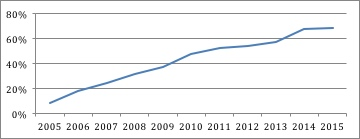
\includegraphics[width=0.5\textwidth]{plots/maxdiffpop}
\label{fig:pop}
\end{figure}
MaxDiff, Maximum Difference Scaling, is a preference measurement and item scaling method.  In a MaxDiff questionnaire the researcher asks respondents for their best and worst item out of a set, then repeats this choice task. Initially proposed by Louviere et al. ~\cite{louviere1991best}, MaxDiff was first released as a software system in 2004 by Sawtooth Software, a top marketing research software company in North America. Since its release its popularity increased steadily with penetration of the technique now reaching 68\% of all Sawtooth users in 2015 (Figure \ref{fig:pop}). \\

MaxDiff offers benefits over alternative methods. MaxDiff provides more discrimination among items and between respondents on the items than traditional rating scales ~\cite{cohen2004s}. Besides enhanced discrimination, it avoids the scale use bias so problematic with traditional ratings scales (CITE).\\
MaxDiff, while it is a distinct type of choice experiment, is closely related to conjoint. A key difference is that it involves both best and worst choices instead of only one. But in its most common form, MaxDiff may be thought of as a one-attribute CBC study with many levels.  \\
\subsection{Studying More Items with MaxDiff: Survey of Market Research Practitioners}
MaxDiff has proven so useful that market researchers increasingly find reasons to use MaxDiff for a large number of items.  How many is a large number of items?  In their 2007 paper, Hendrix and Drucker described ``large sets'' as about 40 to 60 items, proposing variants to MaxDiff called Augmented and Tailored MaxDiff to handle such large problems ~\cite{hendrix2007alternative}. In their 2012 paper, Wirth and Wolfrath also investigated variants to MaxDiff called Express and Sparse MaxDiff for handling what they described as ``very large sets'' of items ~\cite{wirth2012largeset}.  Very large to these authors meant potentially more than 100 items.  To support their findings, they conducted a study among synthetic robotic respondents with 120 items and a real study among humans with 60 items.\\
For Hendrix and Drucker 40 to 60 items was large, for Wirth and Wolfrath 120 items was very large.  For this current paper, we're referring to huge numbers of items as potentially 300 or more. The motivation of our research is beyond academic curiosity, as marketing researchers are seeking such applications pushing MaxDiff further than it was perhaps ever intended. \\
\begin{figure}[!ht]
\caption{Maximum Number of Items Studied via MaxDiff over Last 12 Months}
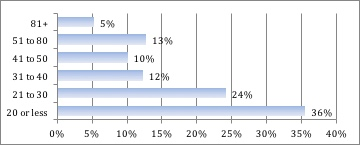
\includegraphics[width=0.5\textwidth]{plots/maxnumstudy}\\
N = ?(TO DO) Mean= 40, Median=30, Maximum=400
\label{fig:max}
\end{figure}
In Sawtooth Software's 2015 Customer Feedback Survey, we asked respondents to tell us the largest number of items they had included in a MaxDiff study during the last 12 months (Figure \ref{fig:max}).  Nearly one-fifth of respondents indicated their firms had conducted a study with 51 or more items.  The maximum number of items studied was 400!\\
To some it may seem bizarre and overwhelming that some researchers are conducting MaxDiff studies with 81+ or even 400 items.  However, when we consider that individual MaxDiff items may actually represent conjoined elements that constitute a profile (say, a combination of packaging style, color, claims, and highlighted ingredients), then it can make much more sense to do 400-item studies.  If the profiles involve multiple highly interactive attributes that pose challenges for CBC, then MaxDiff with huge numbers of items could be a viable alternative (given the new approach we demonstrate further below).\\
\begin{figure}[!ht]
\caption{Main Purpose for MaxDiff Study with 41+ Items}
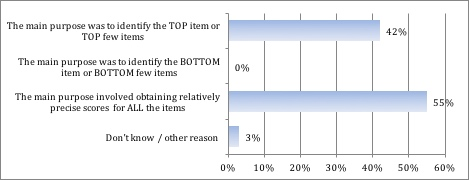
\includegraphics[width=0.5\textwidth]{plots/maxdiffpurpose}
\label{fig:purpose}
\end{figure}
We also asked Sawtooth Software customers what the main purpose was for that study with the reported maximum number of items.  For studies involving 41 or more items, the main reasons are displayed in Figure 3.\\
For 42\% of these large MaxDiff studies, the main purpose was to identify the TOP item or TOP few items.  Our research shows that if this is the main goal, then traditional design strategies are very wasteful.  An adaptive approach using Thompson Sampling can be about 4x more efficient.  Without the Thompson Sampling approach, you are potentially wasting 75 cents of every dollar you are spending on MaxDiff data collection. \\
The problem is that current MaxDiff approaches don't scale well to increasing the number of items.  More items require commensurately longer questionnaires, larger sample sizes, and larger data collection costs with more tired respondents.  If the researcher is concerned about obtaining robust individual-level estimates for all the items, then the current methodologies especially don't scale well to large lists of items.  Respondents just tire out with such long surveys.  In contrast, our approach employs an adaptive divide-and-conquer aggregate approach that leverages prior learning to create more efficient questionnaires and more precise aggregate score estimates. \\
\subsection{Overview of approach: Bandit MaxDiff with Thompson Sampling}
Thompson Sampling has been proposed as an efficient solution for solving the multi-armed bandit problem.  Thompson Sampling involves allocating resources to an action in proportion to the probability that it is the best action ~\cite{thompson1933likelihood}.  Any bandit method must find an appropriate balance between exploring to gain information and exploiting that knowledge.\\
On the one hand, we want to learn about the relative scores of a large number of items within a MaxDiff problem. On the other hand, we want to utilize what we have learned so far to focus our efforts on a targeted set of actions that will likely yield greater precision regarding the items of most interest to the researcher. While there are many methods to accomplish this, Thompson Sampling has proven very useful for these types of problems. For a marketing application of Thompson Sampling and a review of the literature, see Schwartz et al. (2016). \\
The traditional MaxDiff design approach shows each item an equal number of times across all respondents x tasks.  However, if the main goal is to identify the top few items for the sample, after the first, say 20, respondents it seems reasonable to start paying attention to the already-collected MaxDiff responses and oversampling the items that are already viewed as most preferred (the stars).  We can use aggregate logit to estimate both preference scores and standard errors at any point during data collection (say, after the 20th, 40th, $\ldots$. respondent has completed the survey).\\
Thompson Sampling makes a new draw from the vector of item preferences using the estimated population preferences (aggregate logit scores) plus normally distributed error, with standard deviations equal to the standard errors of the logit weights.  As the sample size increases, the standard errors of course tighten.\\
\begin{figure}[!ht]
\caption{Respondent-by-item counts}
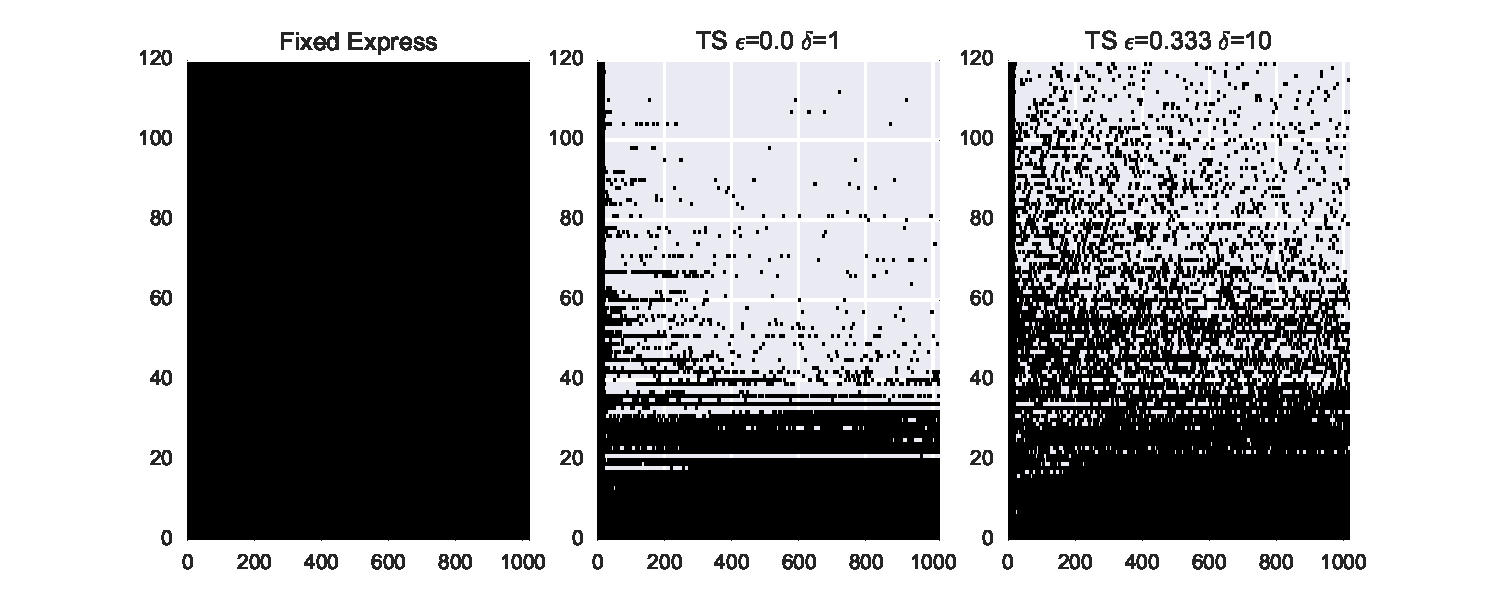
\includegraphics[width=1\textwidth]{plots/3dotplot.pdf}
\label{fig:purpose}
\end{figure}
To understand the logic of the algorithm, consider a snapshot in time during the data collection. Imagine we have just collected data from 100 respondents, and we decide to summarize their preferences (for each of 100+ items) with aggregate logit.  Then, to generate a MaxDiff task for the 101st respondent, we could generate a draw from the population preferences leveraging the population means and normal errors with standard deviations equal to the empirically estimated standard errors.  We then can sort that newly sampled vector of preference scores from the most to the least preferred item.  The five most preferred items might be taken into the first task to show to the 101st respondent.  The process (with or without updating the logit weights after recording the first task's answer) could be repeated to choose the five items to show in the second task for the 101st respondent, etc.  To reduce the load on the server managing the data collection, perhaps only after every 20th respondent has completed the survey, the logit weights and standard errors would be updated.\\
We note that the translation of MaxDiff into a bandit problem is not obvious. Our goal is identifying the utilities of the top set of items with maximum precision. Selecting an arm corresponds to including it in the survey for the next respondent. The reward, however, is not as clear. On the one hand, suppose each task included all possible items. Then the reward would be clear: whether the item is chosen as the ``best.'' But it is not feasible to show so many items to respondents, so that's not a relevant scenario. On the other hand, given we only select a subset of items, the item receiving the ``best'' label doesn't translate directly to a reward. Indirectly, that choice data does enable us to infer how it ranks among all items, exactly aligning with our goal. We use the alignment of the managerial goal and the MAB algorithm's balancing of learning and earning to our advantage. \\
\section{Specifically Bandit + Conjoint = Thompsons + MaxDiff}
\subsection{Thompson Sampling}
\subsection{Eps-Diffuse Thompson Sampling}
We formalize the proposed procedure in three stages. First, we introduce MaxDiff as a best-worst scaling discrete choice task, and we relate it to the standard multinomial logit model. Next, we introduce Thompson Sampling as the natural method of resolving the learn-vs-earn tradeoff as in a multi-armed bandit problem.  Then we generalize that Thompson Sampling algorithm to be more robust by sampling a proportion of items from a more diffuse distribution.
\subsection{MaxDiff choice model}
Every respondent selects both the best and the worst option from an available set of options in each discrete choice task. The model for that data comes from a class of probability models known as best-worst scaling, and MaxDiff is one such model. We adopt the framework from the best-worst scaling literature. For a review, see ~\cite{marley2012models} Marley 2010, ~\cite{marley2005some}. 
We have K possible items, and we select a set S for each choice task. To describe the items, we define two random variables, best $B_z$ and worst $W_z$, for each $z \in S$.  We then define a third random variable, best-worst $BW_{r,s}$, for any $r,s \in S$.\\
Following a random utility framework, these utilities have deterministic and stochastic components.\\ 
A consistent extreme value random utility model is a Thurstone random utility model where each $e_z$ has the extreme value distribution. Consistent model means $B_z=-W_z=U_z$ and $BW_{r,s}=U_r-U_s$, then
\begin{align*}
&B_z=v_z+\epsilon_z\\
&W_z=-v_z-\epsilon_z\\
&BW_{r,s}=v_r-v_s+\epsilon_r-\epsilon_s\\
\end{align*}
We can write the probability that an item is the best and the probability that the item is the worst. 
\begin{align*}
&B_S (x)= Pr⁡( B_x=\max_{z \in S} B_z)\\
&W_S (y)= Pr⁡( W_y=\max_{z \in S} W_z)\\
\end{align*}
Without even using the particular utility or scale of items we can derive choice probabilities. In the most general, form we suppose $b()$ and $w()$ are separate interval scales. Then the resulting probability of an item being best or worst is
\begin{align*}
&B_S (x)= \frac{b(x)}{\sum_{z \in S}b(z)}\\
&W_S (y)= \frac{w(y)}{\sum_{z \in S}w(z)}\\
\end{align*}
For any pair of items, $x,y \in S$, we can write the joint probability that $x$ is best and $y$ is worst. However, when considering the best and worst jointly the scales $b$ and $w$ are not separately identified. So we fix their ratio for the same item by setting $w(z)=\frac{c}{b(z)}$. The resulting joint probability is a function of the ratios of scales for pairs of items, 
\begin{align*}
&BW_S(x,y)=Pr(U_x>U_z>U_y | z \in S -\{x,y\}, x\neq y)\\
&BW_S(x,y)=\frac{b(x)/b(y)}{\sum_{r,s \in S, r \neq s}b(r)/b(s)}
\end{align*}
To accommodate the standard utility structure, we let utility $u(z)=\log{(b(z))}$ Then each of the probabilities 
\begin{align*}
&B_X(x)=\frac{e^{u(x)}}{\sum_{z \in X} e^{u(z)}}\\
&W_X(y)=\frac{e^{u(y)}}{\sum_{z \in X} e^{u(z)}}\\
&WB_X(x,y)=\frac{e^{u(x)-u(y)}}{\sum_{r,s \in X, r\neq s} e^{u(r)-u(s)}}
\end{align*}
We can derive the same representation from the random utility model ~\cite{marley2005some}. \\
We can view best-worst choice as a generalization of the classic multinomial logit for the choice of the best only.\\
\subsection{Estimation}
From our perspective as researchers, all of the utilities are unknown. We can estimate the MaxDiff choice model in a variety of ways. One way to do this exactly is to enumerate all possible pairs of items $x$ and $y$ and then we describe their joint probability of being best and worst, which is the probability of being having the largest difference $BW_S(x,y)$. The pairwise approach scales quadratically in the number of items. We adopt an alternative approach, which reflects the literature and practice and is shown to be a near exact approximation ~\cite{cohen2003maximum}. This allows us to estimate the best model and worst model independently, without explicitly estimating the best-worst probability. 
\begin{align*}
&B_S(x)=Pr(B_x=\max_{z \in S}B_z)=\frac{1}{1+e^{X_B \theta+ e_B}}\\
&W_S(y)=Pr(W_y=\max_{z \in S}W_z)=\frac{1}{1+e^{X_W \theta+ e_B}}
\end{align*}
We describe the data for any individual-task combination. Let $Y_{B_S}(z)$ be the binary choice variable, which equals 1 if the item is selected as best in the set $S$, and 0 otherwise. Then $Y_{W_S}(z)$ is the indicator of whether item $z \in S$ is selected as the worst. The design matrix $X_{B_S}$ (of size $|S|$-by-$K$) contains indicator variables taking on value of 1 for each item in the current set $S$ and 0 otherwise. To signal the item as worst, we set $X_{W_S}=-X_{B_S}$, so $X_{W_S}$ contains values of 0 or -1. Taken together, we express the model of the choice data as a multinomial logit with choice probabilities in vector notation as follows,
\[
\begin{bmatrix}
p_b\\
p_w
\end{bmatrix}
=\logit^{-1}(\begin{bmatrix}X_B\\X_W\end{bmatrix}\theta+\begin{bmatrix}e_b\\e_w \end{bmatrix})
\]
The rows in this matrix representation represent every respondent-task-item combination, $N*J*|S|$, repeated twice.  The probability vectors represent the collection of all best and worst likelihoods for each item in each set for all respondents, $[p_b,p_w]=\{B_S(z),W_S(z)|\forall z \in S, \forall S \in MDD_i, \forall i\}$.
The link between the models of best choice and worst choice is the parameter $\theta=\{\theta_1,\ldots,\theta_k \}$. This common parameter vector represents the overall utility of each item $1,\ldots,k$. For a more positive $\theta_k$, the item $k$ has a larger probability of being chosen as best; the more negative, the more likely the item will be chosen as worst.\\
We clarify language about utility, which may diverge from conjoint language or language for multi-attribute profiles. Since $X$ is an indicator, the $\theta$ only represents the utility of item $k$ being included versus excluded. If $\theta_k > \theta_{k'}$, then we say item $k$ is ``more preferred,'' ``more important,'' or simply, ``better.''\\
Due to the sparse nature of MaxDiff for huge numbers of items plus the desire for rapid real time updates, we decided to use aggregate MNL rather than a Bayesian approach.\\
\subsection{Adaptive MaxDiff}
Since we are uncertain about the each parameter value, we continue collecting data. But we do not need to reduce that uncertainty equally for each one.  To translate our current beliefs about parameters into action, we use Thompson Sampling to select which items to present to the next respondent. 
\begin{align*}
&w_k=\int_{\theta}Pr(u_k(\theta)=u^*(\theta)|D)p(\theta|D)d \theta\\
&k \sim \text{multinomial}(w)\\
&\argmax_k u_k^{(g)} u_k^{(g)} \sim p(u|D)
\end{align*}
Discuss relation to the Follow the regularized leader / perturbed leader 
\subsection{Algorithm MaxDiff TS}
\begin{itemize}
\item For respondents n =1,\ldots,initial
\begin{enumerate}
\item Act: select items for MaxDiff design
\begin{itemize}
\item Sample $L$ items from the population 
\item Create and serve MaxDiff questionnaire to next respondent $J$ tasks of $|S|$ Qs=MDDesign($L$,$|S|$)
\end{itemize}
\end{enumerate}
\item For respondents n = initial + 1,\ldots, N
\begin{enumerate}
\item Estimate: update model $p(D|\theta)$
\begin{itemize}
\item Sample model parameters $u_1,\ldots,u_k \sim p(u|D)$
\end{itemize}
\item Value: rank items by utility
\begin{itemize}
\item Rank and take top $L$ subset $u^{(1)},u^{(2)}\ldots,u^{(L)}$
\end{itemize}
\item Act: select items for MaxDiff design
\begin{itemize}
\item Create and serve MaxDiff questionnaire to next respondent $J$ tasks of $|S|$ Qs=MDDesign($L$,$|S|$)
\end{itemize}
\end{enumerate}
\end{itemize}
We follow the algorithm Bandit MaxDiff-TS. After an initial number of respondents, we begin adapting. We update beliefs about the model parameters. We can draw from an exact or approximate posterior distribution. \footnote{In the case of the multinomial logit, we can use MCMC to obtain samples or, as we do in the empirical application, we can sample from asymptotic distribution via MLE implied by the estimated mean and standard errors.}\\
From a single sample of parameter values, we rank the items by utility. We select the top $L$ items, and we generate a MaxDiff design of $J$ best-worst tasks, each with a choice set of $|S|$ items.  We use $L=30$, $J=18$, $|S|=5$ as a default since it is a standard number of items used in MaxDiff studies (Wirth). 
While typical Bayesian or numerical integration methods call for large numbers of draws (or sufficient number) to achieve coverage of the full distribution of parameter values, our  approach relies on the variability of a single sample. There is value in the sample to sample differences in the value of parameters and their relative rank ordering. It allows  \\
The algorithm learns over time to intuitively achieve the goal of identifying the items with truly high utility with high precision. Early on, we still have substantial uncertainty. The independent samples will differ substantially in rank order of item utilities. This yields MaxDiff designs across respondents with less overlap in items. Later, the uncertainty is reduced most around the truly high-utility items. Across independent samples, the ranking of items will be highly correlated near the top of the ranking (but not near the bottom where uncertainty remains large). As a result, the top subset of $J$ items selected converges to the same group for each respondent. \\
There are two practical issues we highlight. First, we want to avoid repeating extremely similar questions to the same respondent. A natural consequence of Thompson Sampling is convergence: as the sample size grows, items that are most preferred by the population will achieve high preference scores with smaller standard errors.  Without any additional restrictions, the same few items will eventually tend to be drawn into adjacent MaxDiff tasks for the same respondent, causing much annoyance due to the severe degree of item repetition.  Although this is statistically most efficient, it would drive human respondents mad.  To avoid this, we use Thompson Sampling to draw a fixed number of items (e.g., 20 or 30) to show each respondent.  Those draws of 30 items are shown to each respondent in a balanced, near-orthogonal design, leading to a palatably low degree of repetition of items across adjacent sets.  The attentive reader will notice that our approach is quite similar to Wirth's Express MaxDiff approach, except that the logic for selecting the 30 items for each respondent is adaptive, using Thompson Sampling, leveraging information from the previous respondents-focusing the most recent respondent's efforts on discriminating among items that already have been judged likely to be the stars.\\
One issue this approach avoids is the respondent tiring out. Instead of trying to create a MaxDiff design with 120 items, which would lead to an unreasonable number of best-worst tasks per respondent, we use the smaller subset of 30.  We also avoid repetition. A particularly annoying alternative is to draw an independent Thompson sample ranking for each choice task for the same respondent. This results in very repetitive choice tasks as parameter estimates. \\
The second practical issue with Thompson Sampling is robustness to changes overtime. On the one hand, there is built-in robustness. Recall the algorithm is stochastic and adapts continuously. If the early data leads the algorithm astray, then it will self-correct, eventually finding and converging to the truly best items. Suppose the early respondents made choices, by chance, leading us to believe certain items were the best when they were not. The respondents that immediately follow will start receiving these truly poor items. \\
However, as this continues, the uncertainty is reduced around these poor items to reveal there are many other items with probability of being better. By sampling from the joint belief distribution of item utilities, we will be less likely to draw those poor items. One concern is that such sampling could be too aggressive.\\
\subsection{Algorithm MaxDiff $\epsilon$-Diffuse TS}
Perhaps the natural parameter uncertainty is not enough or is perhaps too slow to adjust, so we propose an algorithm MaxDiff epsilon-diffuse TS, which has an extra layer of self-correction, making it more robust to non-stationarity or respondent self-selection. 
The way the $\epsilon$-$\delta$ version hedges its bets on the best items intuitively. As in illustration, instead of sampling 30 items from TS, we use 20 of the items drawn using standard Thompson Sampling (L=30,$\epsilon$=1/3), and 10 of the items drawn using Thompson Sampling with a much more diffuse prior (variance of estimate multiplied by $\delta$=10).
For e-d case, its density does not become a spike as quickly as it does without e-d. This speed is controlled through two parameters: epsilon, the proportion of items sampled from the diffuse distribution, and $\delta$, factor increasing variance for the diffuse distribution.  The larger the $\epsilon$ and $\delta$, the more exploration and slower the algorithm settles on its set of items. The epsilon comes from the popular epsilon-greedy.
The e-d generalization is just like a two-component mixture model, which nests a pooled model without segments. As the epsilon is zero, the diffuse distribution is never used, so the algorithm collapses to regular TS. As $\delta$ is 1, the diffuse distribution is equivalent to the non-diffuse distribution. 
\subsection{Algorithm MaxDiff epsilon-Diffuse TS}
\begin{itemize}
\item For respondents n =1,\ldots,initial
\begin{enumerate}
\item Act: select items for MaxDiff design
\begin{itemize}
\item Sample $L$ items from the population 
\item Create and serve MaxDiff questionnaire to next respondent $J$ tasks of $|S|$ Qs=MDDesign($L$,$|S|$)
\end{itemize}
\end{enumerate}
\item For respondents n = initial + 1,\ldots, N
\begin{enumerate}
\item Estimate: update model $p(D|\theta)$ to obtain population-level estimates, $\bar{u}$ and $\Sigma$.
\begin{itemize}
\item Diffuse TS: Sample model parameters from diffuse distribution, by using rescaled larger variance-covariance $\delta \Sigma$, with $\delta > 1$ \[ u_D \sim N(\bar{u},\delta \Sigma)\]
\item Regular TS: Sample model parameters \[u_R \sim N(\bar{u},\Sigma)\]
\end{itemize}
\item Value: rank items by utility
\begin{itemize}
\item Take top $\epsilon L$ items ranked diffuse sample $u_D^{(1)},u_D^{(2)}\ldots,u_D^{(\epsilon L)}$
\item Take top $(1-\epsilon)L$ items ranked regular sample $u_R^{(1)},u_R^{(2)}\ldots,u_R^{((1-\epsilon)L)}$
\item Combine diffuse and regular samples into $L$ items. (Remove duplicates items. Take the next best unique item from the diffuse sample not already selected.)
\end{itemize}
\item Act: select items for MaxDiff design
\begin{itemize}
\item Create and serve MaxDiff questionnaire to next respondent $J$ tasks of $|S|$ Qs=MDDesign($L$,$|S|$)
\end{itemize}
\end{enumerate}
\end{itemize}
\subsection{Main Empirical Analysis}
We compared our proposed bandit MaxDiff approaches to existing non-adaptive fixed MaxDiff design strategies using simulation based on inferred preferences from an actual MaxDiff survey. We used MaxDiff data from a survey conducted by Procter \& Gamble with Sawtooth Software. The study involved 981 respondents and 120 items from a sparse MaxDiff study. The subject matter and exact item text was hidden for confidentiality purposes. They provided us with the individual-level posterior mean utilities for all respondents and items, which were obtained via Markov Chain Monte Carlo sampling for a hierarchical Bayes (HB) logit model. We call those individual-level utilities the true HB utilities.  These HB utilities offered realistic patterns of preferences across the items and respondents for use in our respondent simulations.  Our simulated respondents mimicked the actual respondents' preferences, on average: to answer each new MaxDiff task, we perturbed those true HB utilities by iid Gumbel error.  \\
For each sample of simulated respondents, we ran aggregate logit and compared the current rank order of the estimated aggregate item scores to the true rank order for the known true utilities.  We define hit rate to reflect how accurately we could recover the top few items as observed in the true preferences for the Procter \& Gamble dataset.  To stabilize the hit rate results (since there was a random component to the responses), we ran the simulations each 100 of times. \\
We used two hit rate measures.\\ \textbf{Top 3 hit rate}: what percent of the top 3 true items the estimated scores using robotic respondents identified.\\ \textbf{Top 10 hit rate}: what percent of the top 10 true items the estimated scores using robotic respondents identified.  For instance, if the estimated scores identified 7 of the true top 10 items (irrespective of order), the hit rate was 70\%.\\
Hit rate is analogous to regret in a typical bandit problem. It measures how far we are from always selecting the truly best arm for all time periods. Although it is not exactly an observed reward in the sense of the usual bandit setting (e.g., clicks, purchases), this serves as the measure of success, \textit{ex post}.\\
\begin{figure}[!ht]
\caption{Distrubution of True Utilities}
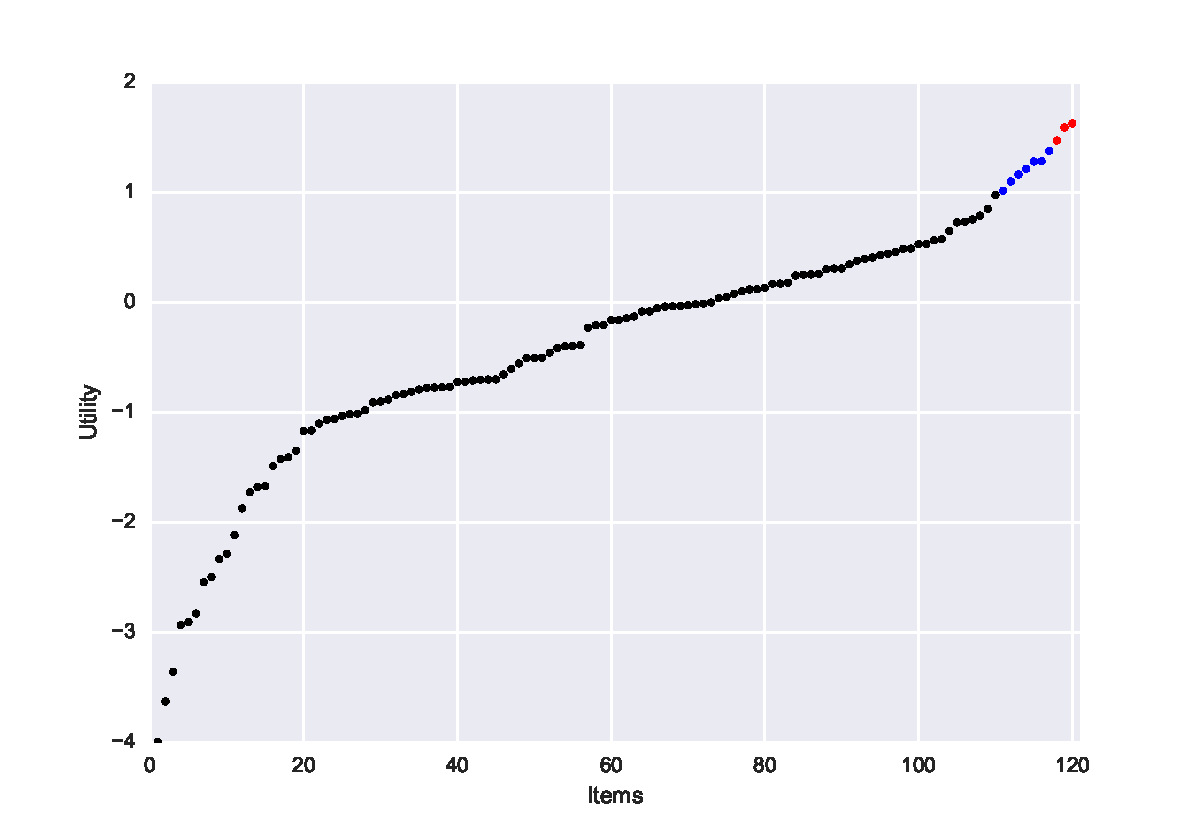
\includegraphics[width=1\textwidth]{plots/utilscore.pdf}
\label{fig:util}
\end{figure}
The difficulty of identifying the truly best items is related to the differences among those top item utilities. With 120 items in the dataset, it shouldn't surprise us if the true preferences for the top 15 or so items were very close in terms of utility.  We certainly observed that with this dataset (Figure \ref{fig:util}).  Due to how tightly the top items in preferences clustered (there were no runaway winners), the hit rate measures we employed were quite discriminating between competing methods.\\
Using bootstrap sampling (sampling with replacement), we simulated the process of collecting respondent data up to sample sizes of $N=1020$.  We considered the first 20 respondents to be the initial group, and all adaptive methods only begin after the 20th respondent. Each robotic respondent completed 18 choice sets, where each set included 5 items, which was viewed as fairly typical of larger MaxDiff studies in practice.
The MaxDiff approaches we tested were the following. For our actual implementation of Bandit MaxDiff, we used Thompson Sampling to draw 30 of the 120 items for each respondent (tending to oversample the ``stars'' based on aggregate logit estimates from previous respondents).  As described earlier, we tested two different Bandit Maxdiff approaches:\\
Bandit MaxDiff TS: All 30 items drawn via standard Thompson Sampling.\\
Bandit MaxDiff epsilon-diffuse TS: We begin with $\frac{1}{3}-\frac{2}{3} $split ($\epsilon=\frac{1}{3}$, $\delta$=10). So 20 of the items drawn using standard Thompson Sampling; 10 of the items drawn using Thompson Sampling with a much more diffuse prior (standard errors multiplied by 10). We also tested a pair of existing fixed MaxDiff approaches.\\
\textbf{Fixed Sparse MaxDiff}: we showed each item to each respondent an equal number of times (if possible).  With 120 items, 18 sets, and 5 items per set each item appeared on average $\frac{18*5}{120} = 0.75$ times per respondent. \\
\textbf{Fixed Express MaxDiff}: we randomly drew 30 of the 120 items to show to each respondent.  Each item appeared $\frac{18*5}{30} = 3$ times per respondent.  Across respondents, each item appeared the same number of times. We primarily use Express MaxDiff as our base case.\\

\begin{figure}
\caption{3 Hit Rate with 120 items}
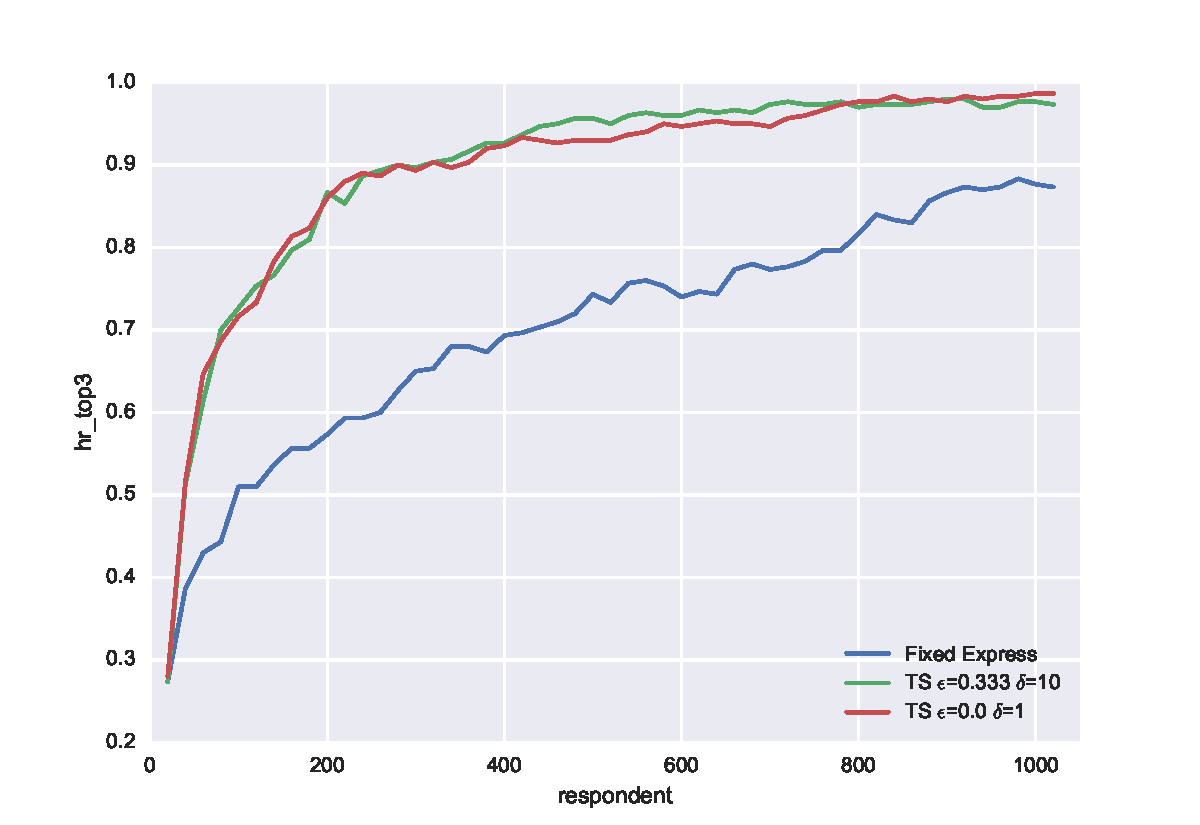
\includegraphics[width=1\textwidth]{plots/3hitrate120show3.pdf}
\label{fig:3hit}
\end{figure}
\begin{figure}
\caption{10 Hit Rate with 120 items}
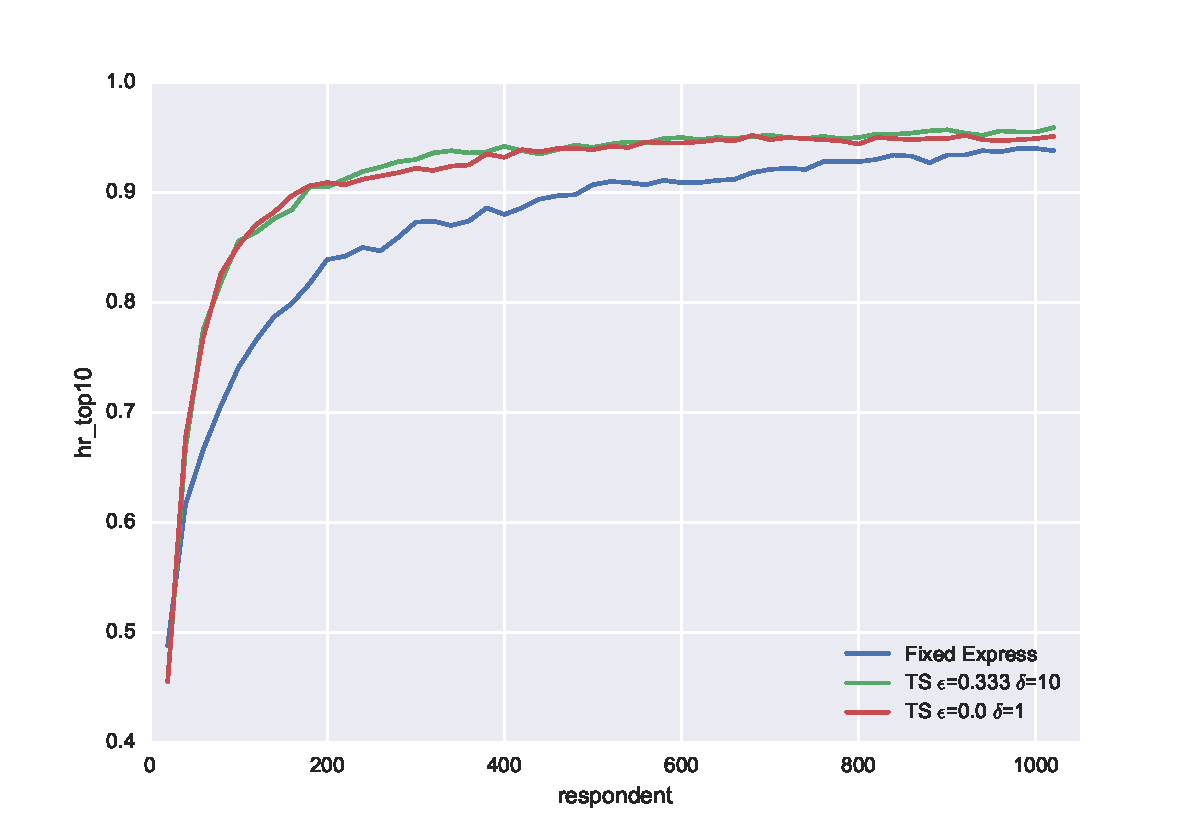
\includegraphics[width=1\textwidth]{plots/10hitrate120show3.pdf}
\label{fig:10hit}
\end{figure}
Figure \ref{fig:3hit} shows the results for the 120-item dataset.  The X-axis indicates the number of cumulative respondents interviewed, and the Y-axis reports the hit rate obtained at each cumulative sample size.  For example, after the first 200 respondents, the Fixed Express Design obtains a hit rate of less than 60\% whereas both Bandit MaxDiff approaches achieve a hit rate of about 85\%.\\
The key takeaway from Figure \ref{fig:3hit} is simple: Thompson Sampling is about 4x more efficient than the standard Fixed Express MaxDiff approach.
\begin{table}
\begin{center}
\begin{tabular}{l | c | c | c}
 Respondent& Fixed Express &  TS $\epsilon$=$\frac{1}{3}$ $\delta$=10  &TS $\epsilon$=0 $\delta$=1 \\
\hline
60&43&61.33&64.67\\
100&51&72.67&71.67\\
160&55.67&79.67&81.33 \\
200&57.33&86.67&86\\
260& 60&89.33&88.67\\
300& 65&89.67&89.33\\
360&68&91.67&90.33\\
400& 69.33&92.67&92.33\\
460&71&95&92.67 \\
500& 74.33&95.67&93\\
560&76&96.33&94\\
600&74&96&94.67\\
660& 77.33&96.67&95\\
700& 77.33&97.33&94.67\\
760&79.67&97.33&96.67\\
800& 81.67&97&97.67\\
860&83&97.33&97.67\\
900&86.67&98&97.67 \\
960&87.33&97&98.33\\
1000& 87.67&97.67&98.67\\
\hline
\end{tabular}
\end{center}
\caption{Top 3 Hit Rate for Various Algorithms}
\label{table:top3}
\end{table}
 We show in Table \ref{table:top3}. After about 160 respondents, we've obtained an 80\% hit rate; which we wouldn't achieve with traditional Express MaxDiff until about the 800th respondent.  As shown, we can accomplish with about 260 respondents what it takes 1000 respondents to do with Express MaxDiff.  Either comparison shows that you can obtain equally good hit rates using the adaptive Bandit MaxDiff methodology with $\frac{1}{4}$ the sample size.\\
Figure \ref{fig:3hit} also shows the two Thompson Sampling approaches achieve nearly identical results. But we will show later this isn't the case if we use a misinformed start (Section Misinformed Start)\\
Figure \ref{fig:10hit} shows the results for Top-10 hit rate for our 120-item MaxDiff, which is a broader measure of success that requires obtaining a high degree of precision for an even broader reach of items than the Top-3 hit rate.  The conclusions are fairly similar as with Figure \ref{fig:3hit}.  It takes about 400 respondents to accomplish with Bandit MaxDiff what we accomplish with 1000 respondents under the non-adaptive express MaxDiff approach. This is supported in Table \ref{table:top3}\\
\subsection{Empirical Evidence of TS Focusing on Top Items}
%\begin{figure}
%\caption{Utility: Mean and 90\% Interval}
%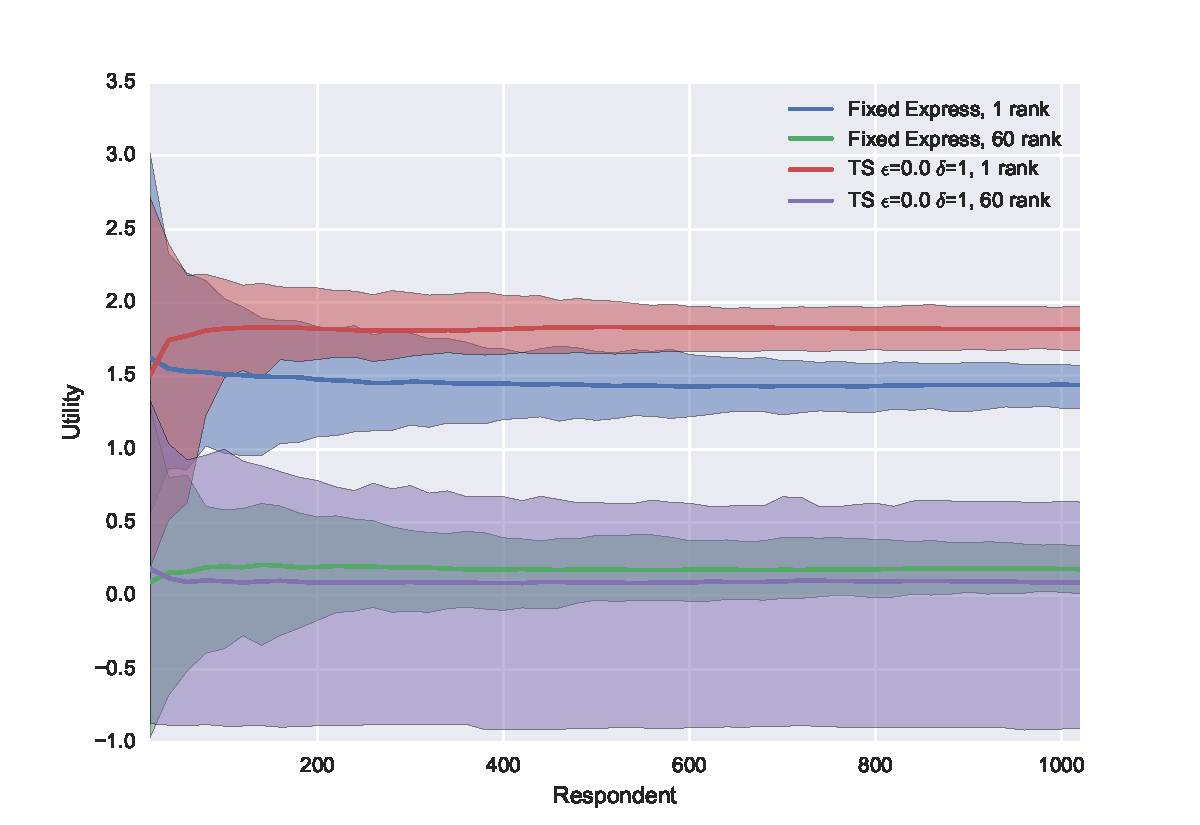
\includegraphics[width=1\textwidth]{plots/betavalconfidence.pdf}
%\label{fig:utilcof}
%\end{figure}
\begin{figure}
\caption{Precision}
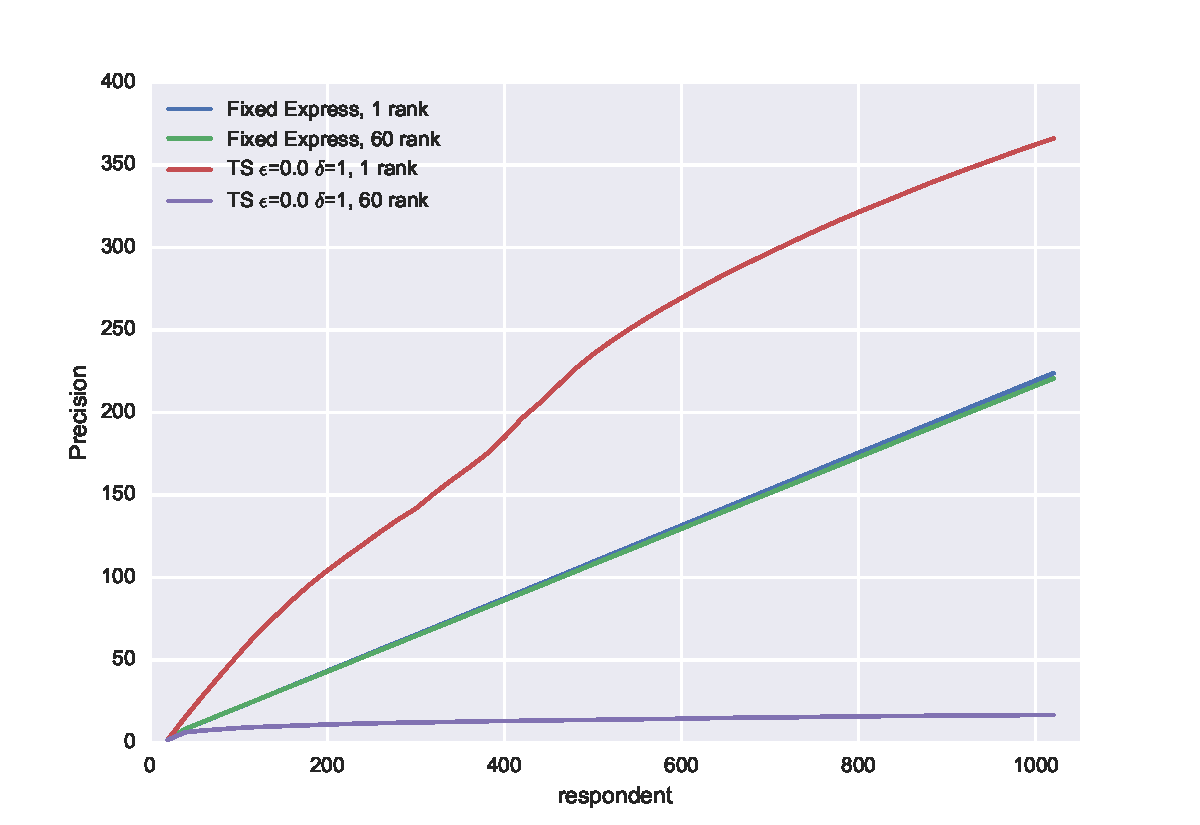
\includegraphics[width=1\textwidth]{plots/precision.pdf}
\label{fig:per}
\end{figure}

\begin{figure}[!ht]
\caption{Distrubution of Utility Belief Distribution}
\begin{subfigure}{.5\textwidth}
\caption{At 120th Respondent}
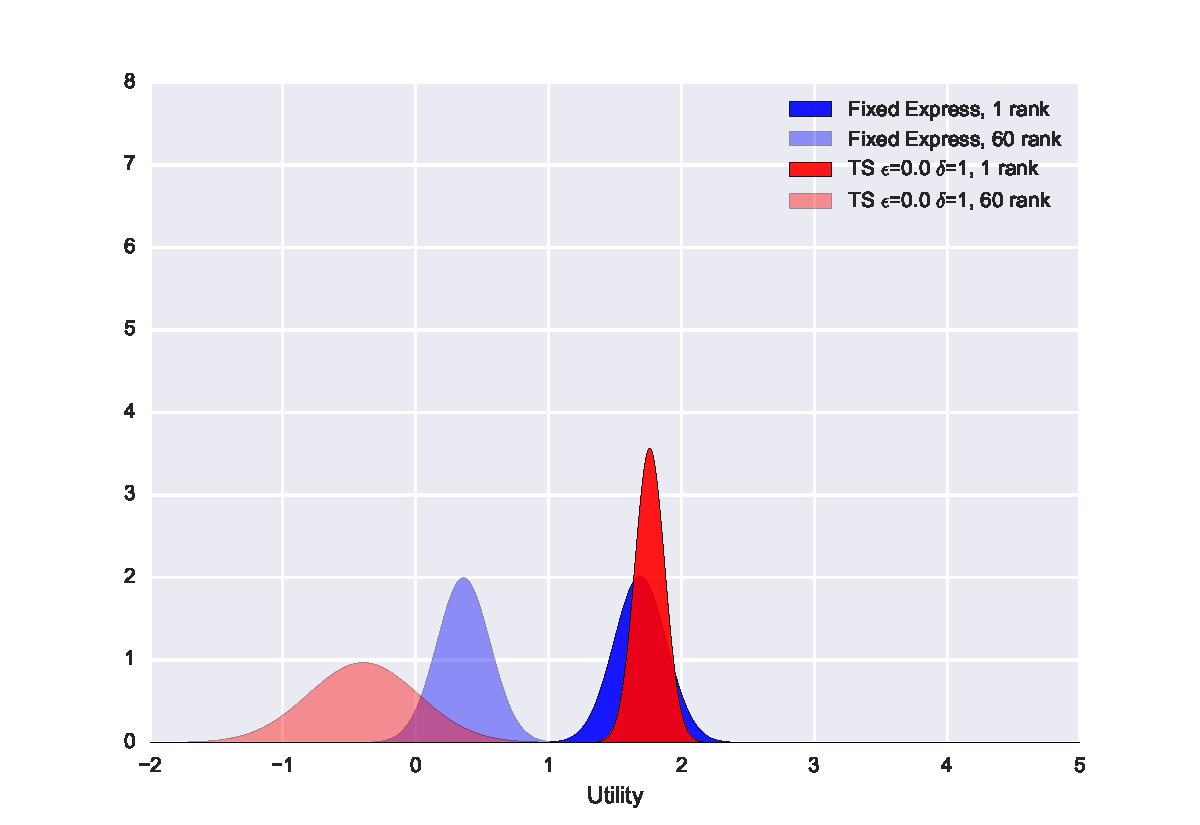
\includegraphics[width=1\textwidth]{plots/beliefdistrBegin.pdf}
\end{subfigure}
\begin{subfigure}{.5\textwidth}
\caption{At 1020th Respondent}
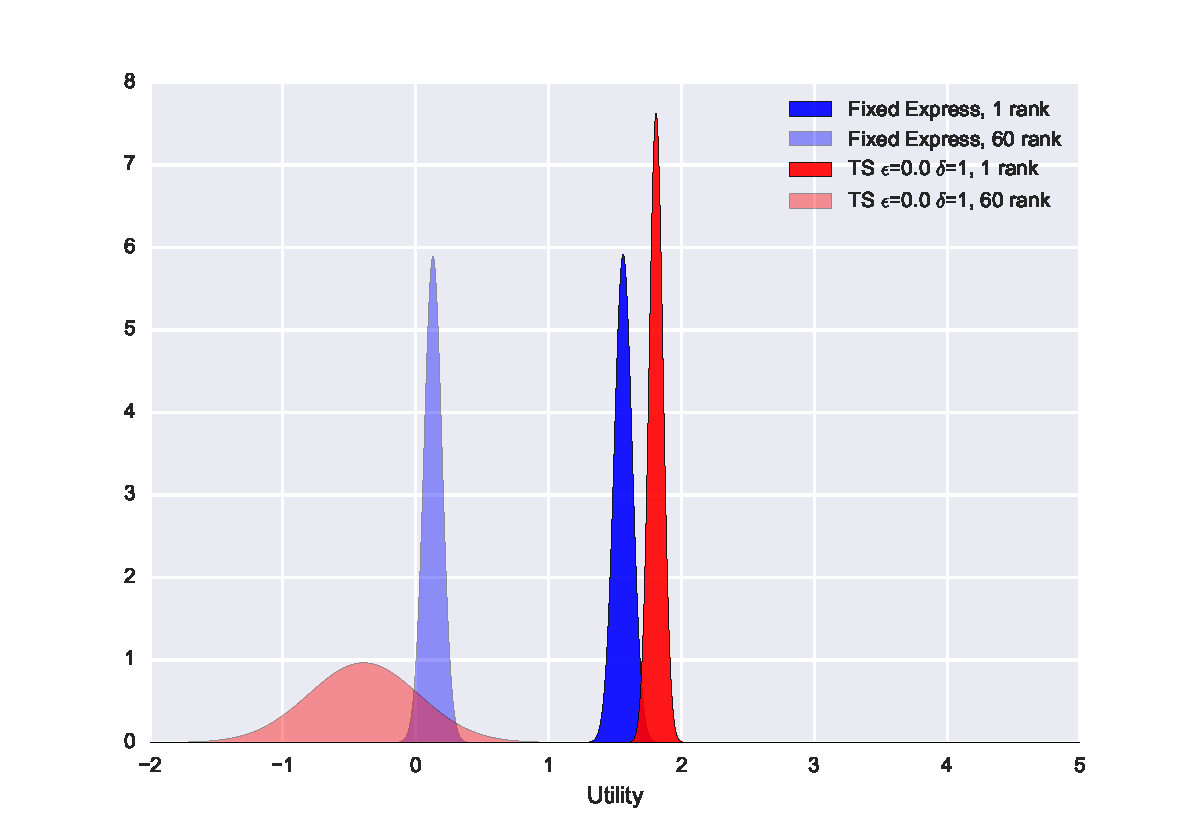
\includegraphics[width=1\textwidth]{plots/beliefdistrEnd.pdf}
\end{subfigure}
\label{fig:belief}
\end{figure}
Figures \ref{fig:per} and \ref{fig:belief} show between the 120th and 1020th respondent the rank 60 item gets almost no update from TS while TS has a large precision on rank 1 item, while Fixed Express updates them both equally as evidence to our claim why TS works well in this context, TS increases the precision a lot on the higher ranked items of those items while not learning the lower ranked items while Sparse Express spends its resources equally.

%\begin{figure}[!ht]
%\caption{Distrubution of Final Utility}
%\begin{subfigure}{.5\textwidth}
%\caption{Rank 1 Item}
%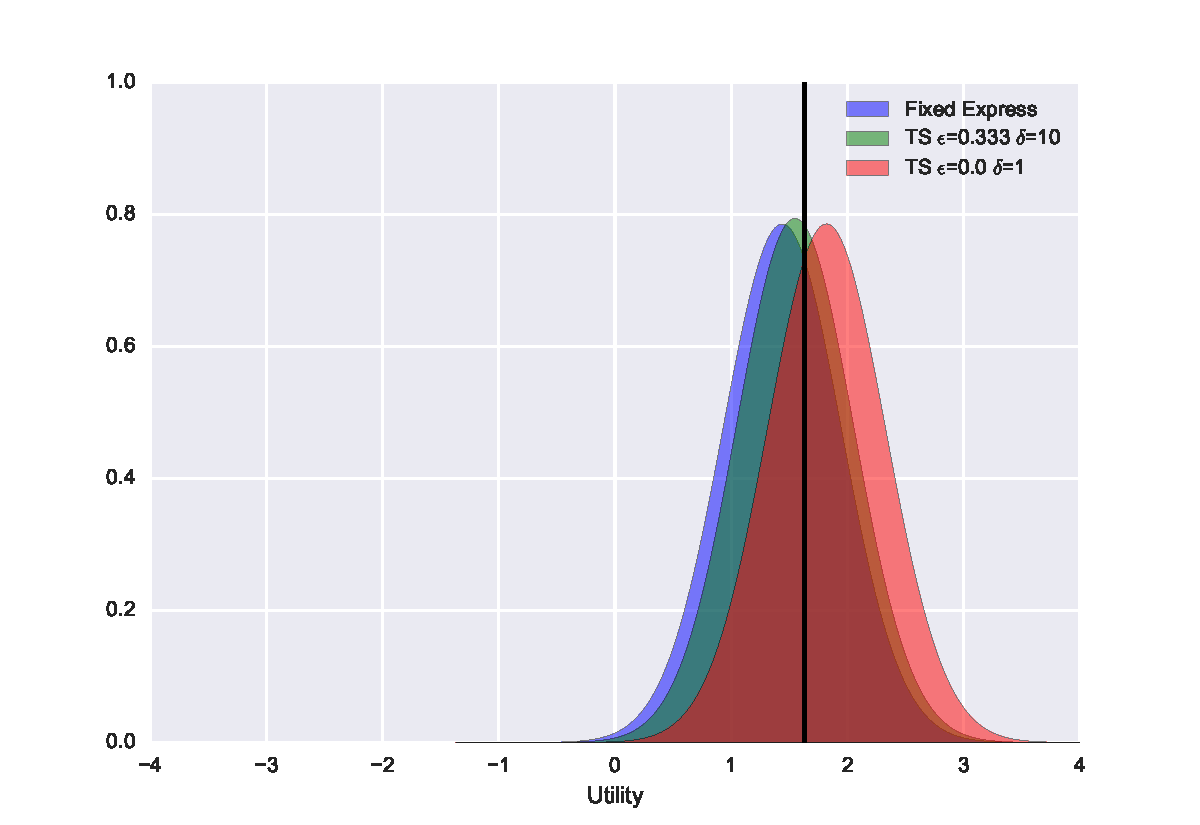
\includegraphics[width=1\textwidth]{plots/endbetadis1.pdf}
%\end{subfigure}
%\begin{subfigure}{.5\textwidth}
%\caption{Rank 30 Item}
%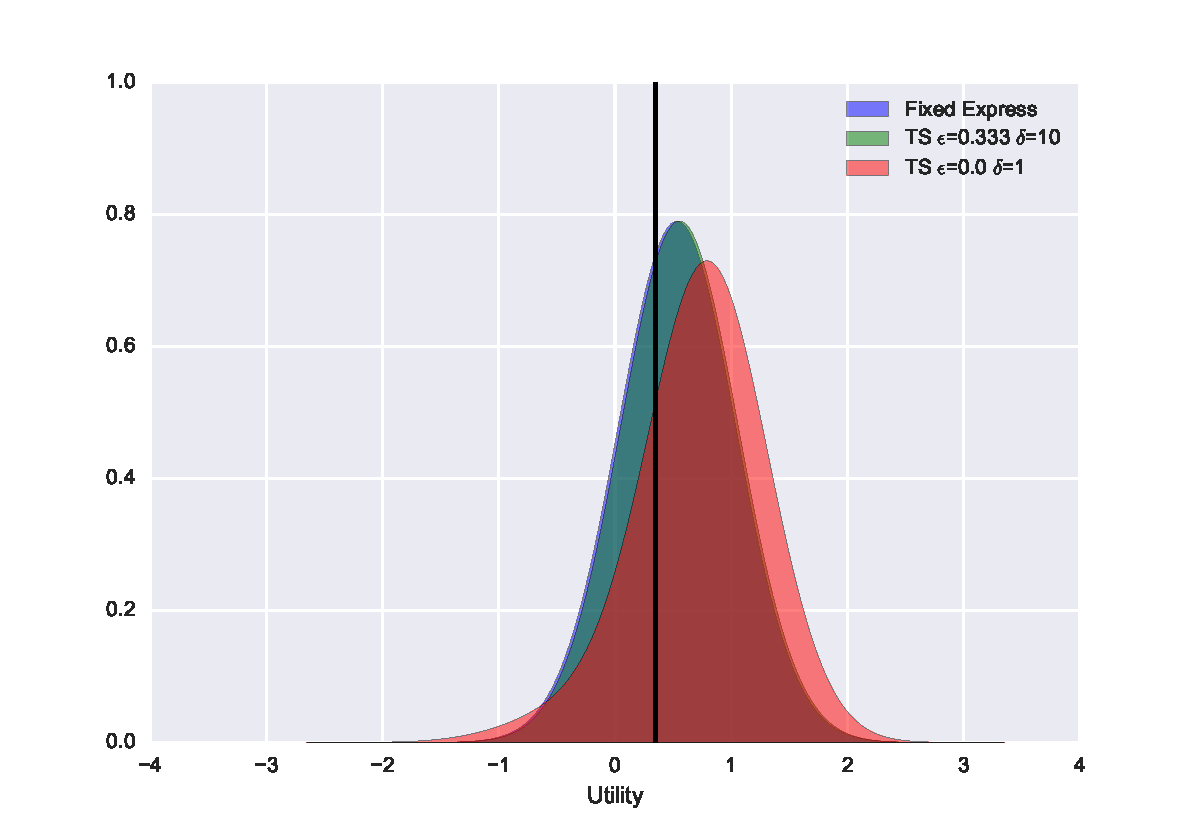
\includegraphics[width=1\textwidth]{plots/endbetadis30.pdf}
%\end{subfigure}
%\begin{subfigure}{.5\textwidth}
%\caption{Rank 60 Item}
%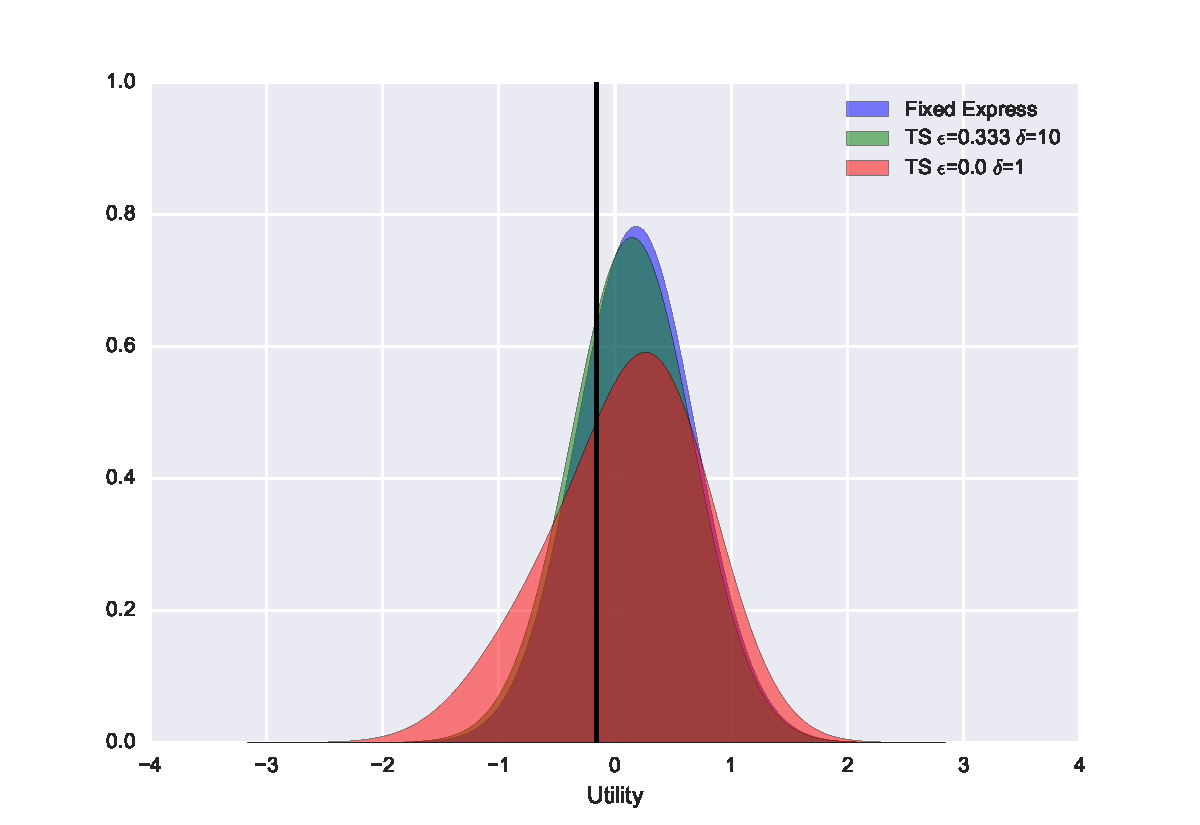
\includegraphics[width=1\textwidth]{plots/endbetadis60.pdf}
%\end{subfigure}
%\begin{subfigure}{.5\textwidth}
%\caption{Rank 90 Item}
%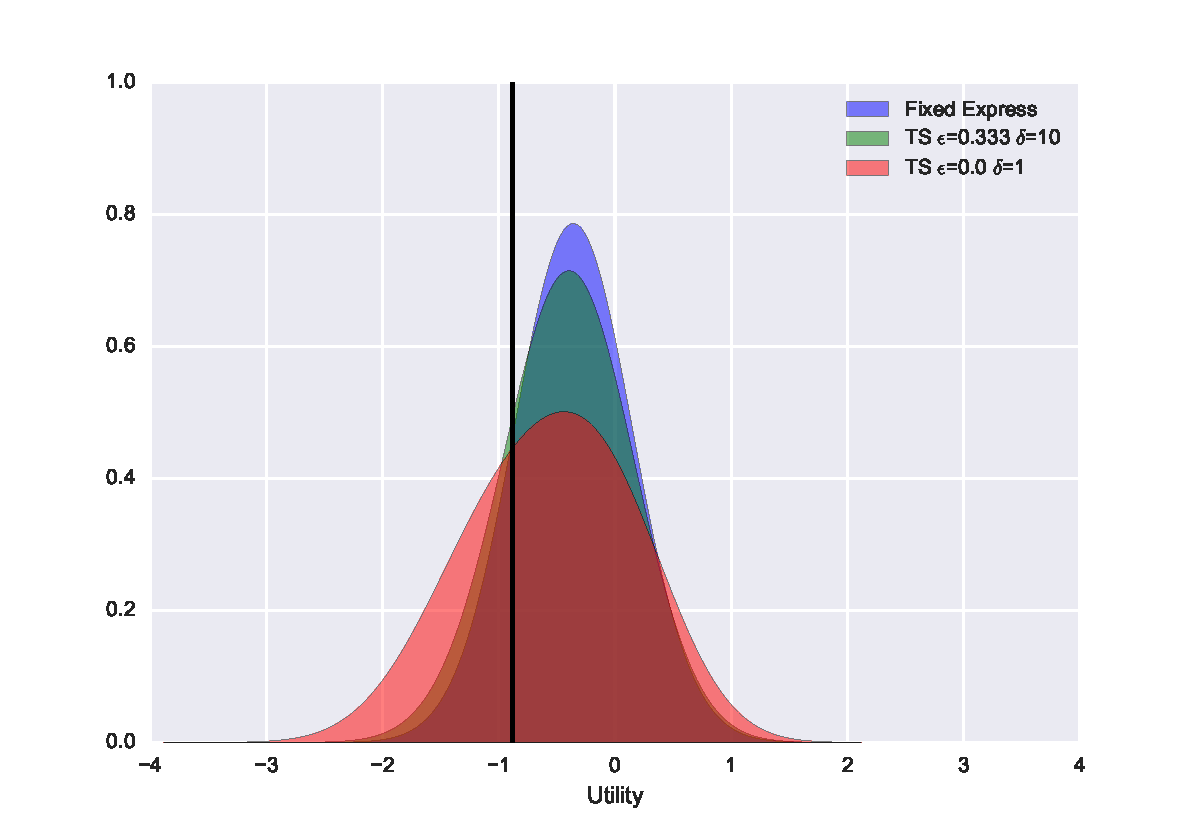
\includegraphics[width=1\textwidth]{plots/endbetadis90.pdf}
%\end{subfigure}
%\label{fig:end}
%\end{figure}
\section{Robustness tests}
\subsection{Misinformed Starts (When Early Responders Are Horribly Non-Representative)}
To this point, it seems like the adaptive Bandit MaxDiff approach using Thompson Sampling is the clear winner.  However, what would happen if the first 50 respondents we interviewed were actually not very representative of the average preferences for the sample?  What if we tried to throw Bandit MaxDiff off the scent?  In fact, let's consider a worst-case scenario: the first responders actually believe \textit{nearly the opposite} from the rest of the sample\\
For the simulations reported in Figure 6, the first 50 robotic respondents mimicked randomly drawn human vectors of utilities as before but were diabolically manipulated to behave as if the top 3 true items were actually nearly the worst in preference (we set the utilities for the top 3 true items for the population equal to the bottom 25th percentile utility item for each respondent).  After this misinformed start, the remaining respondents represented well-behaved respondents drawn using bootstrap sampling as before, with true individual-level preferences as given in the original dataset donated by Procter \& Gamble.\\
Our diabolical simulation of a misinformed start is worse than anything you would realistically see in practice, so it is a strong test of the robustness of the Bandit MaxDiff approach. This suggests robustness to non-stationarity in preference or self-selection of respondents during the sampling window. We created 50 misinforming early responders because in practice we are never guaranteed that the first responders represent a fair and representative draw from the population.  In fact, depending on how rapidly we invite a panel of respondents to take the survey, the first 50 respondents may share some atypical characteristics (e.g. anxious and available to take the survey at your launch time).  It would be a bad thing if the Thompson Sampling approach performed well in simulations with well-behaved respondents, but fell apart under more realistic conditions. \\
\begin{figure}
\caption{3 Hit Rate with 120 items with Misinformed Start}
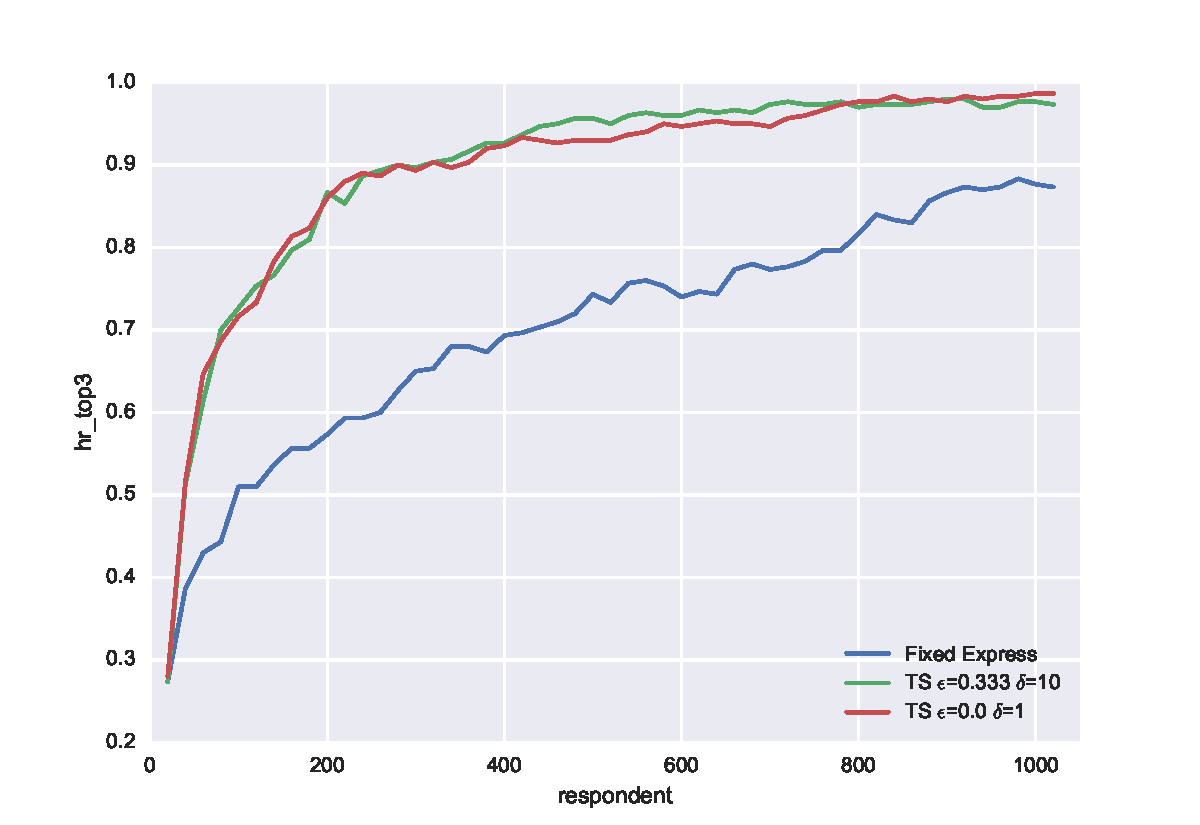
\includegraphics[width=1\textwidth]{plots/3hitrate120show3.pdf}
\label{fig:3hitmis}
\end{figure}
We illustrate the robustness in Figure \ref{fig:3hitmis}. First, the Bandit MaxDiff $\epsilon$-diffuse TS approach is much better in the face of misinformed starts than the standard Bandit MaxDiff TS approach.  The more diffuse prior on the 10 out of 30 items within the split allows us to continue investigating the value of some lesser chosen items with enough frequency among later respondents, even if the prior respondents seem to have generally rejected them.\\
Second, even in the face of a misinformed start, the Bandit MaxDiff $\epsilon$-diffuse TS achieves equally good results as the standard Express MaxDiff without the misinformed start after 290 respondents. Finally, the conclusions were qualitatively similar when examining Top-10 hit rate.\\
\subsection{Changing exploration parameters}
\begin{table}
\begin{center}
\begin{tabular}{l | c | c | c | c | c }
 Respondent& TS $\epsilon$=0 $\delta$=1&  TS $\epsilon$=$\frac{1}{3}$ $\delta$=10  &TS $\epsilon$=$\frac{1}{3}$ $\delta$=20 & TS $\epsilon$=$\frac{1}{2}$ $\delta$=10 &TS $\epsilon$=$\frac{1}{2}$ $\delta$=20  \\
\hline
100	&	71.67	&	72.67	&	74	&	74.67	&	71.33	\\
200	&	86	&	86.67	&	84.67	&	89.67	&	82.67	\\
300	&	89.33	&	89.67	&	92.67	&	94	&	91.33	\\
400	&	92.33	&	92.67	&	94	&	97.33	&	95.33	\\
500	&	93	&	95.67	&	98.67	&	98.33	&	96.33	\\
600	&	94.67	&	96	&	99.33	&	99	&	97.33	\\
700	&	94.67	&	97.33	&	98.67	&	98.67	&	96.67	\\
800	&	97.67	&	97	&	99	&	98.67	&	98.33	\\
900	&	97.67	&	98	&	99	&	98.33	&	98.67	\\
1000	&	98.67	&	97.67	&	98.67	&	99.33	&	98.33	\\
\hline
\end{tabular}
\end{center}
\caption{Top 3 Hit Rate for Various Tuning Parameters}
\label{table:EDTS}
\end{table}
We introduced two tuning parameters– $\epsilon$ and $\delta$ –  into an algorithm that previously had no such parameters explicitly guiding exploration. To understand the impact these exploration parameters have and each one's effect on the outcome, we have to test their values empirically. \\
We run a simulation experiment with a 5-cell design 2($\epsilon=\frac{1}{3}, \frac{1}{2}$)-by-2($\delta$=10,20) + 1($\epsilon$=0,$\delta$=1).  The standard TS has $\epsilon=0$and $\delta=1$, but either one . Recall that the fixed express MaxDiff is equivalent to $\epsilon$=1 and $\delta\inf$, rendering any parameter distribution to be uninformative, as it is effectively uniform.\\
Table \ref{table:EDTS} shows how these parameters can affect performance; these effects, however, are small. The best performing combinations are $\epsilon=\frac{1}{2}$,$\delta$=10 and $\epsilon=\frac{1}{3}$,$\delta$=20. This suggests there is an ``interior solution,'' as there are non-monotonic effects of the exploration parameters. There is a value of epsilon, which makes edTS better than TS, and the same is true for delta. This pattern is consistent with empirical implementations of epsilon-greedy strategies. In fact, the table shows the best performing algorithm tested uses only one exploration parameter set high, and the worst performing algorithm tested has both parameters set to their higher-exploration level.\\

\subsection{Effect of increasing number of items}
\begin{table}
\begin{center}
\begin{tabular}{l | c | c | c}
 Respondent& Fixed Express &  TS $\epsilon$=$\frac{1}{3}$ $\delta$=10  &TS $\epsilon$=0 $\delta$=1 \\
\hline
100	&	22.33	&	44.33	&	47.67	\\
200	&	31	&	70	&	67	\\	
300	&	41.33	&	76	&	72	\\	
400	&	42.67	&	79	&	78.33	\\	
500	&	46.33	&	85.33	&	79.33	\\
600	&	48	&	89.33	&	82	\\	
700	&	53.67	&	88.67	&	85.67	\\
800	&	54.67	&	90.67	&	86.33	\\
900	&	55.67	&	91.33	&	88	\\
1000	&	59	&	91.33	&	89	\\	
\hline
\end{tabular}
\end{center}
\caption{Top 3 Hit Rate for Various Algorithms with 300 items}
\label{table:300top3}
\end{table}
Would the benefits of Bandit MaxDiff we observed with 120 items continue for 300 items?  While we didn't have a dataset of utilities from human respondents on 300 items, we did our best to generate such a data set by leveraging the 120-item data set Procter \& Gamble shared with us.  To generate preferences across an additional set of 180 items, we randomly combined pairs of existing items according to a randomly distributed weighting scheme, with additional random variation added.  The result was a 300-item MaxDiff data set based on the original preferences of the 981 respondents.\\
Our results for both well-informed and misinformed starts were nearly identical to the 120-item results.  Table \ref{table:300top3} shows the consistent results. The Bandit MaxDiff approach was again 4x more efficient than the standard Express MaxDiff approach on the top-3 hit rate criterion. \\
\subsection{What about a smaller set of 40 Items?}
\begin{table}
\begin{center}
\begin{tabular}{l | c | c | c}
 Respondent& Fixed Express &  TS $\epsilon$=$\frac{1}{4}$ $\delta$=10  &TS $\epsilon$=0 $\delta$=1 \\
\hline
60	&	71.33	&	81	&	84.33	\\
100	&	79.33	&	88	&	89.33\\
160	&	86.33	&	93	&	93.33	\\
200	&	91	&	95.67	&	94.67	\\
260	&	92.67	&	96.33	&	96.33	\\
300	&	94.33	&	96.67	&	97	\\
360	&	94.67	&	98.33	&	98	\\
400	&	94.33	&	98	&	98.33	\\
460	&	94.67	&	99	&	99	\\
500	&	95.33	&	99.33	&	98.33	\\
\hline
\end{tabular}
\end{center}
\caption{Top 3 Hit Rate for Various Algorithms with 300 items}
\label{table:40top3}
\end{table}
Our Bandit model has a great advantage over fixed designs for very large numbers of items, but what happens if we have a more traditional ``large'' MaxDiff list of 40 items. Using a random 40-item subset from our original set of 120 items, we reran our simulations. For this smaller subset, we also reduced the number of tasks per respondent to 12 and we drew 20 items per respondent using TS rather than 30 items and used a 15/5 split between standard TS and diffuse TS.\\
By reducing the number of items to 40 and changing the number of tasks to 12, the fixed express design can now show each item an average of 1.5 times per respondent, which is much less sparse than in larger item cases.\\
Nevertheless, our results for Bandit MaxDiff are still much better than traditional MaxDiff (Table \ref{table:40top3}). We see about a 2x efficiency gain compared to the Sparse MaxDiff. We also still see a tremendous advantage in the case of a misinformed start.\\
\subsection{Using True Utility as a Generalization of Hit-Rate}
Say an algorithm gets the top 9 items and the 11th item in the 10 top items. One might like to differentiate that between another algorithm that gets the top 9 items and the 40th item in the 10 top items is Percent True Utility. \\
\textbf{Exponetial Weighted Utility}: For a set $S$ the exponential weighted utility is \[\mu_S=\sum_{x \in S}b(x)=\sum_{x \in S}e^{u(x)}\]
\textbf{Percent True Utility of the Top 3 (or 10)}: The exponential weighted true utility of the top 3 (10) items that the robotic respondents identified over the maximum exponential weighted true utility that could be attained with 3 (10) items. Mathematical if $S^*$ is the top 3 (10) items and $S$ is the current 3 (10) top items identified robotic respondents then Percent True Utility is 
\[
\frac{\mu_S}{\mu_{S^*}}
\]
This can be see as a Generalization of Hit-Rate though it has the advantage of differentiating as in the case above. Though one loses the ability to easy interpret the result . 
\begin{figure}
\caption{Percent True Utility of the Top 3 with 120 items}
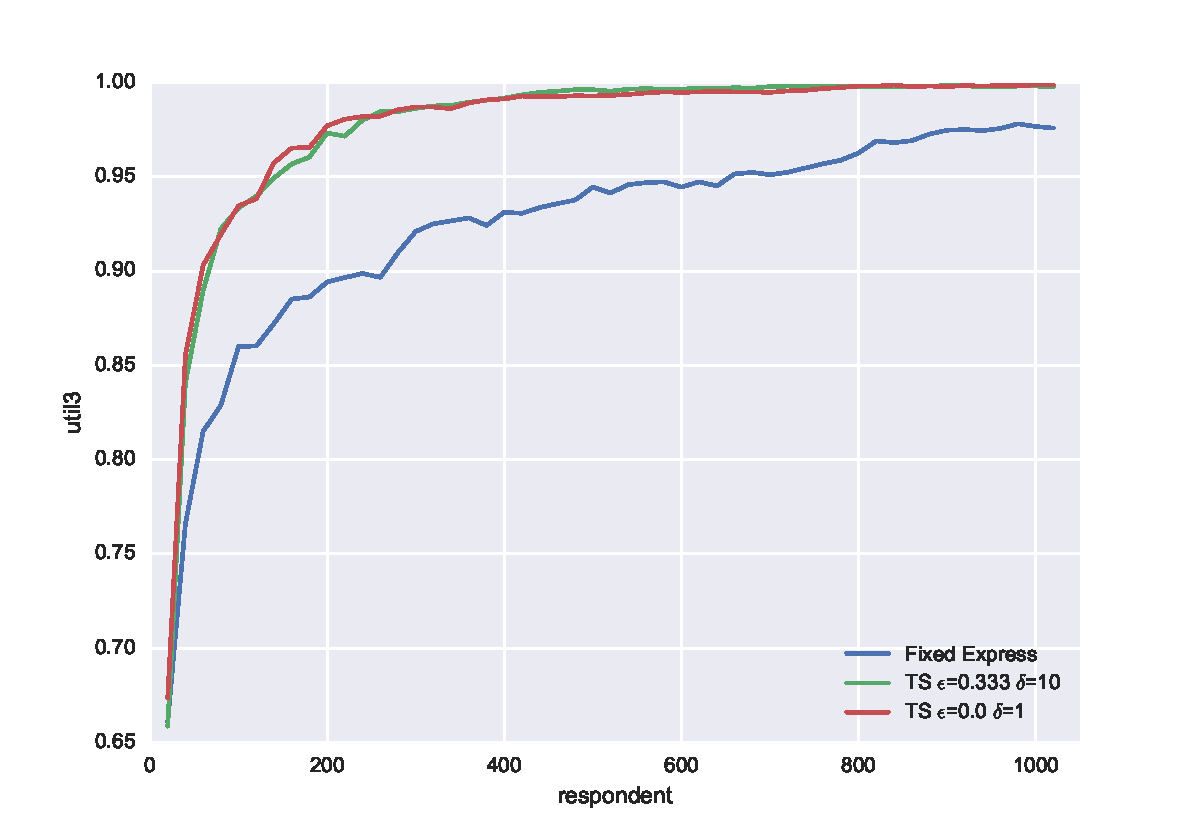
\includegraphics[width=1\textwidth]{plots/3util120show3.pdf}
\label{fig:3util}
\end{figure}
In Figure \ref{fig:3util} Percent True Utility tells a similar story to Hit Rate.

\subsection{Using Regret as a Stopping Rule}
In practice we do not know the True Utilities \textit{a priori} but we would like to know 
Taken from ~\cite{scott2015multi} and ~\cite{scott2010modern} for MAB, The value remaining in the experiment is the posterior distribution of $\frac{\mu_{S^*}-\mu_{S}}{\mu_{S}}$ where $\mu_{S^*}$ is the largest value of the exponential weighted utility and $\mu_{S}$ is the exponential weighted utility of the set that is most likely to be optimal denoted $S$. This is constructed as follows, take $n$ Monte Carlo draws from $p(\mu|y_t)$. Let $\mu_{S^*}^{m}$ be the max exponential weighted utility of draw $m$ and $\mu_{S}^{m}$ be the utility using the draw $m$ using the set $S$. Let $\Delta^{m}=\frac{\mu^m_{S^*}-\mu^m_{S}}{\mu^m_{S}}$.\\
\begin{table}
\begin{center}
\begin{tabular}{l | c c c c c c c c}
Current & 1st &  2nd  &  3rd  &  4th &  5th & 6th & 7th &  8th \\
\hline
Draw 1 & 4.02 &  3.50 &  5.08 & 4.16&  4.22 & 4.41 & 3.65 &  3.27 \\
Draw 2 &4.18 & 4.72 & 3.49 & 3.48 & 3.63 & 3.60 & 3.56 &  3.70 \\
Draw 3 &4.81 & 5.23 & 5.04 &  3.96 &  4.17 & 4.37 &  3.58 & 2.99 \\ 
\end{tabular}
\end{center}
\caption{Draws of the exponetial utility of the items after 100 iterations}
\label{table:data}
\end{table}

\begin{figure}
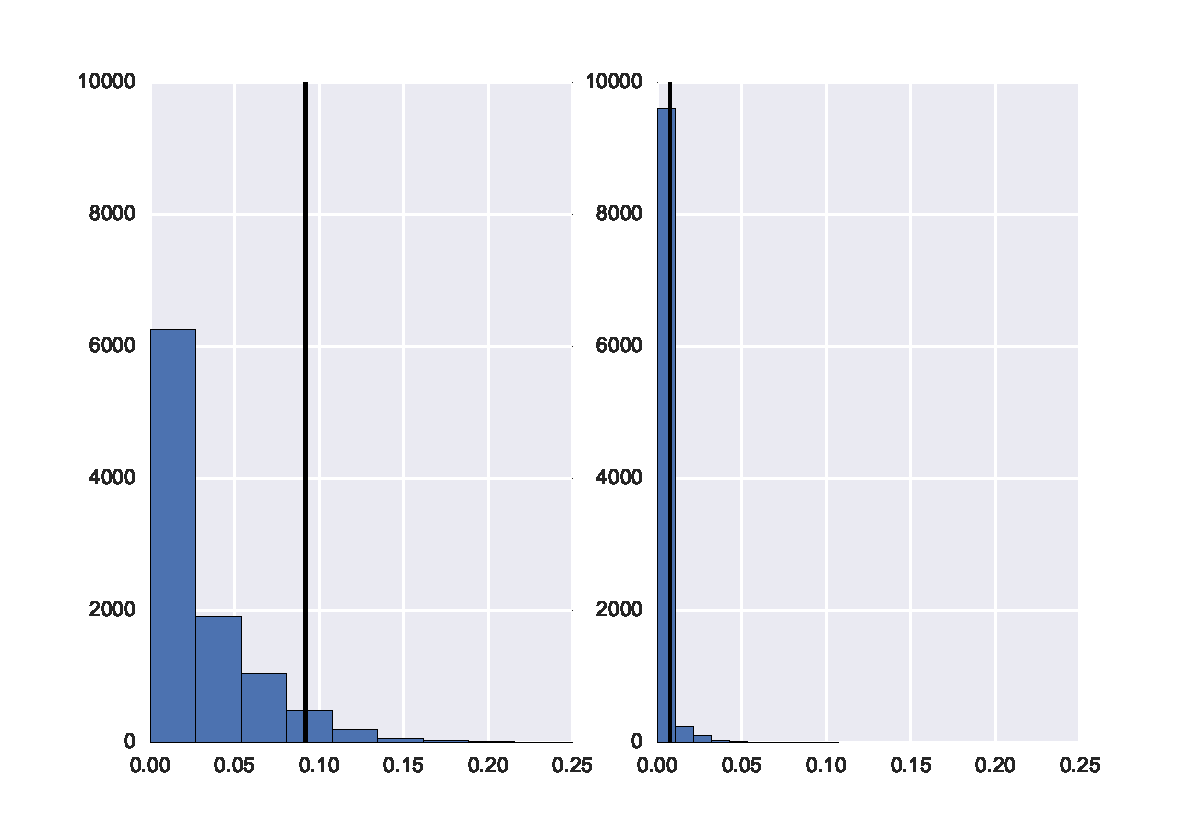
\includegraphics[width=1\linewidth]{plots/valremhist.pdf}
\caption{Two histograms of $\Delta$. Left: After 100 iterations, the potential value remaining is .092. Right: After 220 iterations, the potential value remaining is .008}
\label{fig:data}
\end{figure}

As an example I took draws after respondent 100 in TS $\epsilon=.67$ $\delta=10$ for 120 items see table \ref{table:data} for draws of exponential weighted utility of a single item. I put the columns in current rank order and only show the top 8 for convenience. Say we were finding the value remaining for the the utility score using the top 3. Then $S=\{1,2,3\}$. Then $\mu^1_{S}=4.02+3.50+5.08=12.6$ and $\mu_{S^*}^{1}=5.08+4.41+4.16=13.65$ So $\Delta^{1}=\frac{13.65-12.6}{12.6}=.083$. Likewise $\Delta^{2}=\frac{12.6-12.39}{12.39}=.017$ and $\Delta^{3}=\frac{15.08-15.08}{15.08}=0$ (Note $\Delta^m=0$ when the $S$ contains the top utilities). The histogram of $\Delta$ after 100 iterations and 220 iterations is shown in figure \ref{fig:data}. \\
 The `potential value remaining' (PVR) is the .95 quantile of the distribution $\Delta$ which in this case was .092. A way to interpret this number is ``We do not know what the utility of $S$ is, but whatever it is, a different set might beat it by as much as 9.2\%.''\\
 A good stopping rule is to stop when the PVR drops below a certain threshold, (We use .02). One advantage of this is it handles ties (two sets with close exponential weighted utility scores) really well. 
\begin{figure}
\caption{Potential Value Remaining of the Top 3 with 120 items}
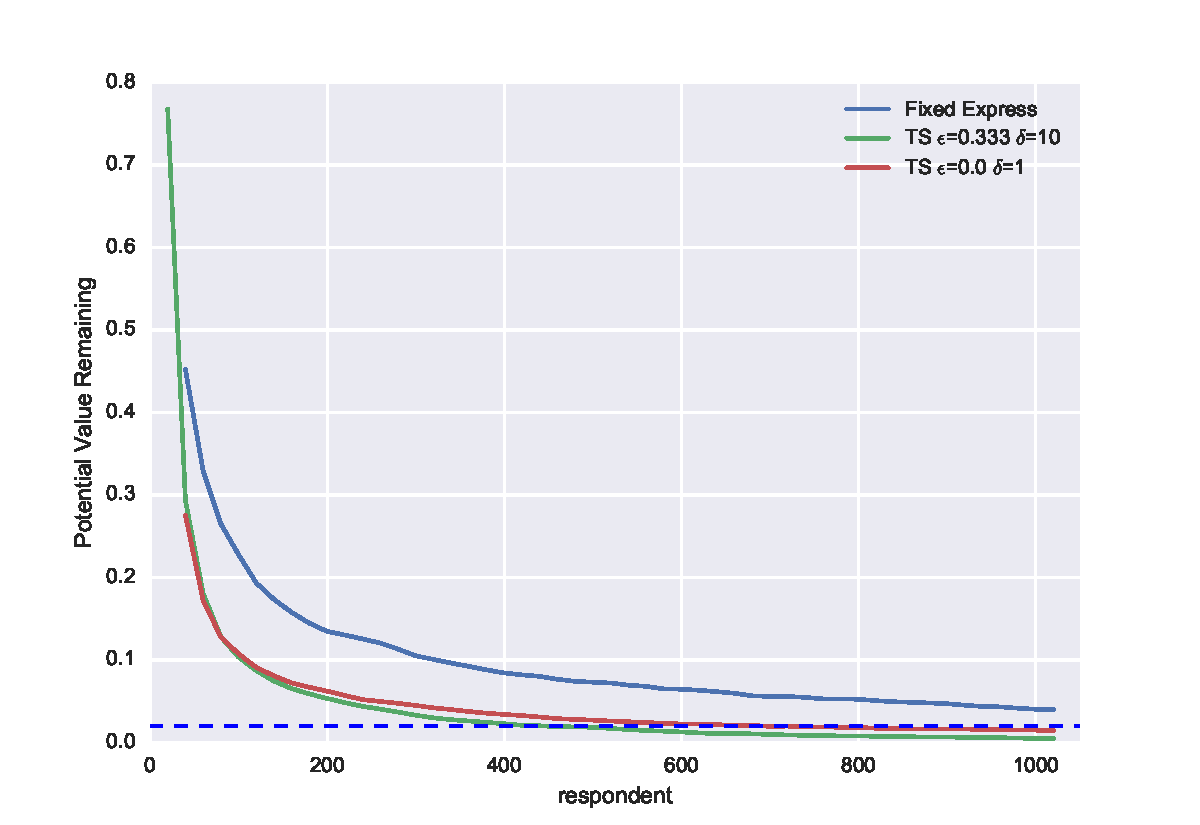
\includegraphics[width=1\textwidth]{plots/3vr120show3ex.pdf}
\label{fig:3vr}
\end{figure}
\begin{figure}
\caption{Histogram of When Iterations Would Stop Using a .02 Stopping Rule}
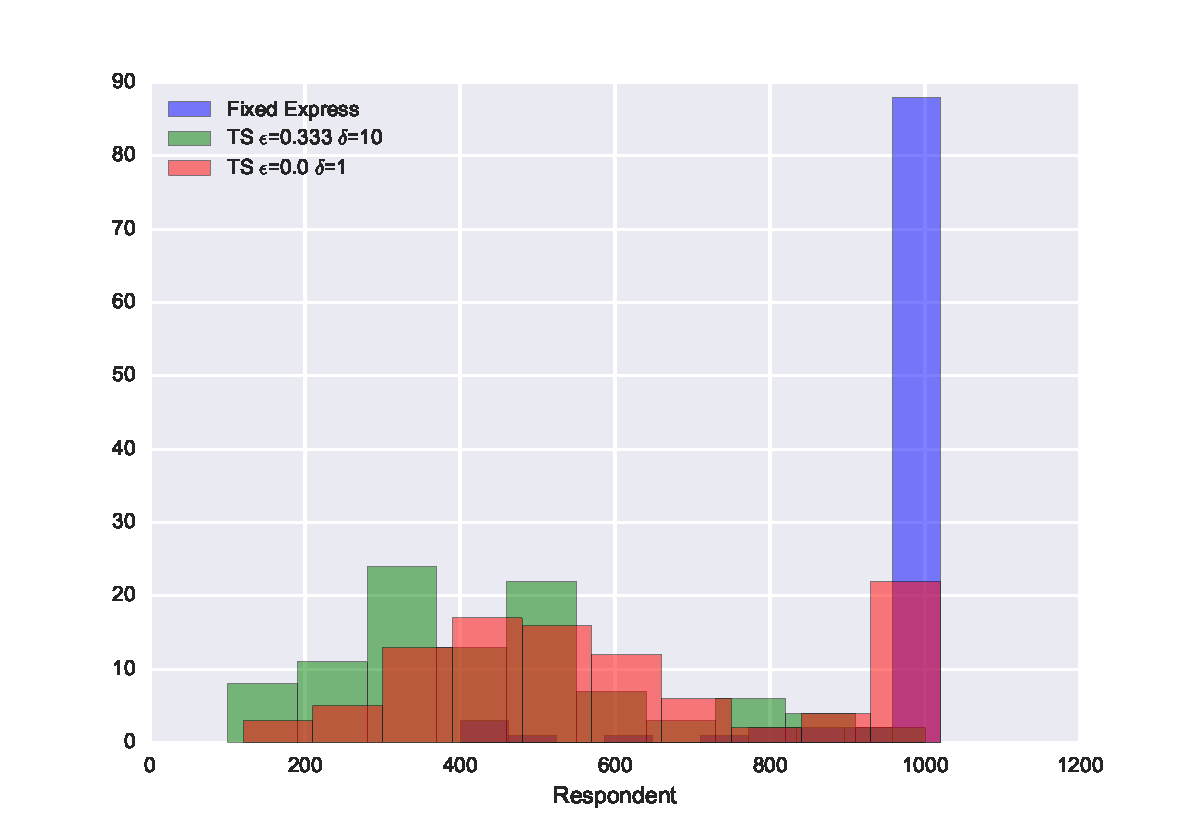
\includegraphics[width=1\textwidth]{plots/stop120items23.pdf}
\label{fig:3vrhist}
\end{figure}
\begin{figure}
\caption{Percent True Utility of the Top 3 When Iteration Stops}
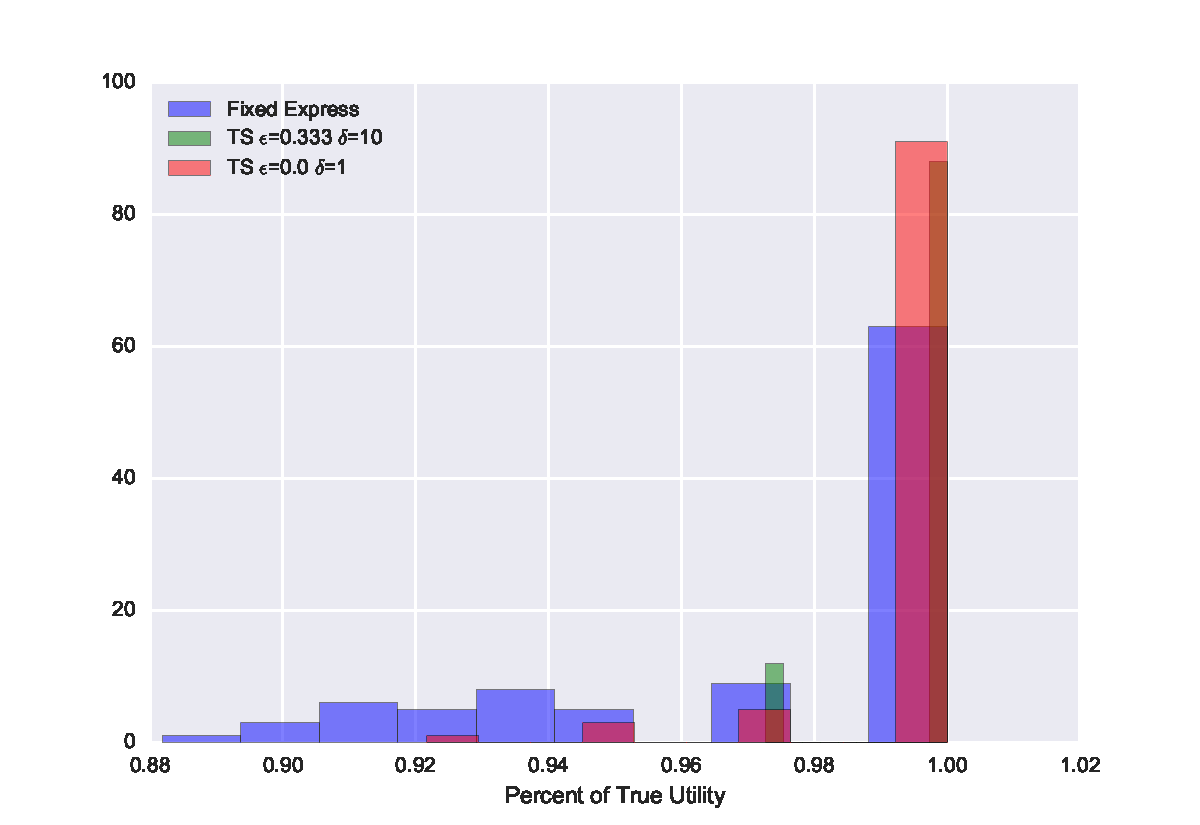
\includegraphics[width=1\textwidth]{plots/util120items23.pdf}
\label{fig:3vrutil}
\end{figure}
In Figure \ref{fig:3vr} we see the average PVR using the top 3 items on a log scale. Figure \ref{fig:3vrhist} show on which respondent the iterations' PVR would reach .02 (with the max being 1020)and Figure \ref{fig:3vrutil} shows what the Percent True Utility would be at those points. Another advantage we see for Bandit MaxDiff $\epsilon$-diffuse TS approach is that on average it stops sooner that standard TS with no decrease in performance. Both Bandit MaxDiff TS stop much sooner and preform much better then fixed express.\\
\begin{table}
\begin{center}
\begin{tabular}{l | c | c | c}
 & Fixed Express &  TS $\epsilon$=$\frac{1}{3}$ $\delta$=10  &TS $\epsilon$=0 $\delta$=1 \\
\hline
40 items&&&\\
Mean Stop& 358.6&  190.4 &  201.8\\
Mean PTU&.993 & .997 & .997 \\
\hline
120 items&&&\\
Mean Stop& 980.8 &  440.6 &  606.0 \\
Mean PTU& .976 & .997 & .996 \\
\hline
300 items&&&\\
Mean Stop& 1020.0 &  674.2 &  929.4\\
Mean PTU&.904 & .992 & .988 \\
\hline
\end{tabular}
\end{center}
\caption{Mean respondent each algorithm would stop at and the mean percent true utility (PTU) at that point when a stopping rule at PVR .02 is implemented}
\label{table:stop}
\end{table}
In Table \ref{table:stop} We see the means under different numbers of items. We see the benefits of using $\epsilon$-diffuse TS grow much larger as the number of items increases.
\subsection{Asking for Bests instead of Best-Worst}
Because a key assumption for using the Bandit MaxDiff approach is that the researcher is mainly interested in identifying the top few items, we wondered about the value of spending time asking respondents to identify the worst item within each MaxDiff set.  What would happen if we asked our robotic respondents only to select the best item within each set?  The results somewhat surprised us.  The value of asking respondents to indicate both best and worst within each set more than compensated for the 40\% additional effort we suppose these ``worst'' questions add to the total interview time when interviewing human respondents.
In a five item set (A,B,C,D and E) there are 10 possible 2-way comparisons. If we assume A is preferred to B and B is preferred to C and so on, then asking about only the best item will let us know A$>$B, A$>$C, A$>$D and A$>$E (4/10 comparisons).  By asking about worsts as well, for only one additional question we also add B$>$E, C$>$E, and D$>$E (7/10 comparisons), leaving only the order relationship between B, C, and D unknown.
\subsection{What about Double Adaptivity?}
In 2006, one of the authors presented a paper on Adaptive MaxDiff that featured within-respondent adaptation ~\cite{orme2006adaptive} rather than what we have shown here in Bandit MaxDiff based on Thompson Sampling, which is an across-respondent adaptive approach.  For the within-respondent adaptive procedure, items that a respondent indicates are worst are dropped from further consideration by that same respondent through a round-robin tournament until eventually that respondent's best item is identified.  We thought adding this additional layer of within-respondent adaptivity on top of the Bandit MaxDiff approach could additionally lift its performance.  To our surprise, this double-adaptive approach actually performed worse than Bandit MaxDiff alone in terms of hit rates for the globally best 3 or 10 items for the sample.  After some head-scratching (and much code checking), we determined that the lack of improvement was due to degree of heterogeneity across the robotic respondents.  For example, if we are interviewing a respondent who doesn't agree much with the overall population regarding which are the top items, it is detrimental to allow that respondent to drop from further consideration (due to judging them worst) what actually are among the globally most preferred items.  It serves the greater good for each respondent to spend increased effort judging among the items that previous respondents on average have judged as potentially best.
\subsection{What about Sparse MaxDiff vs. Express MaxDiff?}
Wirth and Wolfrath compared non-adaptive Sparse MaxDiff and Express MaxDiff in their 2012 paper at the Sawtooth Software Conference ~\cite{wirth2012largeset}.  We compared the results using our simulation and found a modest edge in performance for Sparse MaxDiff (Sparse ending at 80\% for top 10 hit rate and express ending at 75\%).
\section{Conclusions and Future Research}
Our results suggest that if your main purpose in using large item lists in MaxDiff is to identify the top items for the population (not individual-level estimates), then adaptive Bandit MaxDiff approaches can be 4x more efficient than standard Express MaxDiff designs.  You are potentially wasting 75 cents of each dollar spent on data collection by not using Bandit MaxDiff.\\
Bandit MaxDiff leverages information from prior respondents to show more effective tradeoffs to later respondents (tending to oversample the stars, based on the Thompson Sampling mechanism).  Even in the face of diabolically imposed misinformed starts (horribly unrepresentative first responders), the Bandit MaxDiff approach with our 20/10 split is extremely robust and self-correcting.\\
Although our simulations involve 120-item and 300-item tests, we expect that even greater efficiency gains than 4x (compared to standard Express MaxDiff designs) may occur with 500-item (or more) MaxDiff studies.  For studies using 40 respondents, our simulation showed a 2x advantage in efficiency over fixed MaxDiff designs. Though not as dramatic, this is still a sizable boost.\\
Future research should test our findings using human respondents.  Using an adaptive process that focuses on comparing best items may result in a more cognitively difficult task than a standard level-balanced, near-orthogonal approach.  The greater expected within-set utility balance may lead to higher response error which may counteract some of the benefits of the Bandit adaptive approach.  However, based on previous research ~\cite{orme2006adaptive} that employed within-respondent adaptivity, the additional degree of difficulty that the Bandit adaptive approach could impose upon individual respondents (owing to utility balance) would probably not counteract the lion share of the benefits we've demonstrated using simulated respondents.\\
We should note that as of this article's publication date, Sawtooth Software does not offer Bandit MaxDiff as a commercial tool.  Sawtooth Software may perhaps one day soon offer Bandit MaxDiff as an option within its commercially available MaxDiff software.  As for the authors, we look forward to this possibility as we've been especially impressed by the potential cost savings and increased accuracy!










% Acknowledgments here
\ACKNOWLEDGMENT{%
% Enter the text of acknowledgments here
}% Leave this (end of acknowledgment)


% Appendix here
% Options are (1) APPENDIX (with or without general title) or 
%             (2) APPENDICES (if it has more than one unrelated sections)
% Outcomment the appropriate case if necessary
%
% \begin{APPENDIX}{<Title of the Appendix>}
% \end{APPENDIX}
%
%   or 
%
% \begin{APPENDICES}
% \section{<Title of Section A>}
% \section{<Title of Section B>}
% etc
% \end{APPENDICES}

% References here (outcomment the appropriate case) 

% CASE 1: BiBTeX used to constantly update the references 
%   (while the paper is being written).
\bibliographystyle{informs2014} % outcomment this and next line in Case 1
\bibliography{source} % if more than one, comma separated

% CASE 2: BiBTeX used to generate mypaper.bbl (to be further fine tuned)
%\input{mypaper.bbl} % outcomment this line in Case 2

\end{document}


